% Papers must not exceed 15 pages total (including the references and appendices).

% Anonymous Submission. Papers must be submitted in a form suitable for
% anonymous review: no author names or affiliations may appear on the
% title page, and papers should avoid revealing their identity in the
% text. When referring to your previous work, do so in the third person,
% as though it were written by someone else. Only blind the reference
% itself in the (unusual) case that a third-person reference is
% infeasible. Contact the program chairs if you have any
% questions. Papers that are not properly anonymized may be rejected
% without review.

\documentclass[10pt, conference, compsocconf]{IEEEtran}

%% Custom TeX

\usepackage{listings}
\usepackage{xcolor}
\usepackage{xspace}
\usepackage{graphicx}
\usepackage{caption}
\usepackage{subcaption}
\usepackage{rotating}
\usepackage{amssymb}
\usepackage{url}
\usepackage[splitrule]{footmisc}

%% for comments
\newcommand{\comment}[3][\color{red}]{{#1{[{#2}: {#3}]}}}
\newcommand{\kris}[1]{\comment[\color{orange}]{km}{#1}}
\newcommand{\jeff}[1]{\comment[\color{green}]{JSF}{#1}}

\newcommand{\thickhline}{\noalign{\hrule height 1pt}}

%% names of things
\newcommand{\fuzzer}{CloakDroid\xspace}
\newcommand{\lib}{Mr.\ Hide\xspace}
\newcommand{\hidelib}{\code{hidelib}\xspace}
\newcommand{\troyd}{\code{troyd}\xspace}
\newcommand{\rewriter}{Dr.\ Android\xspace}

%% Statistics

\newcommand{\numinvestigatedapps}{750\xspace}
\newcommand{\numpointspercity}{10\xspace}
\newcommand{\numappsusinglocation}{275\xspace}
\newcommand{\numcities}{6\xspace}
\newcommand{\numstationaryapps}{261\xspace}
\newcommand{\numfinegrainedapps}{34\xspace}
\newcommand{\code}[1]{\textsf{#1}}
\newcommand{\bcode}[1]{\texttt{#1}}
\newcommand{\coarsenotfine}{???\xspace} % FIXME
\newcommand{\finenotcoarse}{???\xspace} % FIXME
\newcommand{\coarseandfine}{???\xspace} % FIXME
\newcommand{\adsonly}{???\xspace} % FIXME
\newcommand{\listapps}{???\xspace} % FIXME
\newcommand{\weatherapps}{???\xspace} % FIXME
\newcommand{\otherapps}{???\xspace} % FIXME
\newcommand{\cdiff}{\delta}

%%%% Computer generated statistics
\newcommand{\numappsweather}{21\xspace}
\newcommand{\numappsnearbycities}{22\xspace}
\newcommand{\numappsunsure}{17\xspace}
\newcommand{\numappsads}{78\xspace}
\newcommand{\numappsonlyads}{58\xspace}
\newcommand{\numappslist}{43\xspace}
\newcommand{\numappslistads}{6\xspace}
\newcommand{\numappstagging}{28\xspace}
\newcommand{\numappsfinegrained}{34\xspace}
\newcommand{\numappsfinegrainedads}{7\xspace}
\newcommand{\numappstaggingads}{4\xspace}
\newcommand{\numappsweatherads}{2\xspace}
\newcommand{\numappsnottestable}{52\xspace}
\newcommand{\numappsnearbycitiesads}{1\xspace}


\newcommand{\numappsweather}{21\xspace}
\newcommand{\numappsnearbycities}{22\xspace}
\newcommand{\numappsunsure}{17\xspace}
\newcommand{\numappsads}{78\xspace}
\newcommand{\numappsonlyads}{58\xspace}
\newcommand{\numappslist}{43\xspace}
\newcommand{\numappslistads}{6\xspace}
\newcommand{\numappstagging}{28\xspace}
\newcommand{\numappsfinegrained}{34\xspace}
\newcommand{\numappsfinegrainedads}{7\xspace}
\newcommand{\numappstaggingads}{4\xspace}
\newcommand{\numappsweatherads}{2\xspace}
\newcommand{\numappsnottestable}{52\xspace}
\newcommand{\numappsnearbycitiesads}{1\xspace}

%% Apps

\newcommand{\app}[1]{#1}
\newcommand{\hospitals}{\app{Hospitals Near Me}}
\newcommand{\tdbank}{\app{TD Bank}}
\newcommand{\webmd}{\app{WebMD}}
\newcommand{\gasbuddy}{\app{Gasbuddy}}
\newcommand{\restaurantfinder}{\app{Restaurant Finder}}
\newcommand{\walmart}{\app{Walmart}}

%% End of custom TeX

\begin{document}
%
% --- Author Metadata here ---
% --- End of Author Metadata ---

\title{An Empirical Study of Location Truncation on Android}


\maketitle
\begin{abstract}
  Location-based apps are popular on Android, but they raise a number
  of privacy concerns. In this paper, we empirically study how one
  popular location-privacy enhancing technique, location truncation,
  affects app utility. That is, we try to answer the question: How
  much can we truncate the location information given to an app while
  still preserving the app's usability? To this end, we developed
  CloakDroid, a tool that can apply a user-specified amount of
  location truncation to an arbitrary Android app. We then surveyed a
  large set of apps from Google Play and found that many apps use
  location to generate lists of nearby objects. For this category of
  apps, we developed three metrics of the usability of an app's output
  list before and after location truncation: Edit distance between the
  lists; set intersection size, treating the two lists as sets; and
  the additional distance incurred to go to the first (closest) entry
  of the list.  Finally, we used CloakDroid to conduct experiments to
  compute these metrics for six apps across a range of locations (in
  cities varying in population from 6,000 to 8.2 million) and
  truncations (from 0.1~km to 50~km).  We found that the amount to
  which an app's location could be truncated mainly depends on the
  density of objects being measured by the app, and that most apps can
  have their inputs truncated to between 5~km and 20~km without
  significantly degrading app utility.
\end{abstract}

\section{Introduction}
\label{sec:introduction}

Many mobile apps use
location information.
As implemented today, such apps typically send the device
location over the Internet, and hence users may be understandably
concerned about potential privacy violations. In response,
researchers have developed a number of location privacy-enhancing
mechanisms \cite{Beresford:2004, Shokri:2011, Shokri:2012,
Bettini:2005, Hoh:2005, Gruteser:2003},
 using a range of analytical models to estimate the degree of privacy 
and anonymity achieved.

However, there has been much less work \cite{Brush:2010} 
 on understanding
how location privacy-enhancing technology affects the \emph{utility}
of apps---that is, does an app still work well enough even when
location privacy is increased.  In this paper, we tackle this question
by \emph{directly} measuring how \emph{location truncation}---quantizing the
current location to a user-specified grid spacing---changes the output
of a range of Android apps.

Location truncation is one of the more realistic
approaches to location privacy, with several advantages: It is easy
for users to understand and therefore trust.  It can be implemented
easily and efficiently. And it does not require foreknowledge of the
set of locations to be visited. There are also some
disadvantages: Location truncation primary defeats localization
attacks, rather than deanonymization or tracking \cite{Krumm:2009}.
Location truncation may also be overcome through a
combination of prior knowledge (e.g., likely movement speeds,
locations of road networks, known habits, etc) and repeated queries
over a long period of time~\cite{Gruteser:2005} \cite{Krumm:2007}.
Even so, we believe that for many everyday uses, these limitations are
not severe for typical users.

While location truncation potentially increases privacy, it may not be
ideal for all apps (e.g., it defeats turn-by-turn navigation), and its
effects may be hard to measure (e.g., for apps that use location to
decide which ads to show).  We retrieved the top \numinvestigatedapps apps
across all categories of the Google Play store, and found that
\numappsusinglocation of these use location. We ran each app
to determine how and why they use location, and found six main
categories: ad
localization, listing nearby objects, fine-grained tasks (e.g.,
turn-by-turn navigation), geotagging content (such as pictures),
finding the nearest city, and getting local weather information. (See
Section~\ref{sec:usage}.)

Based on this result, we chose to study the effect of location
truncation on apps that produce lists of nearby objects. 
These apps
are a good target for a variety of reasons: First, the effect of
truncation is easy to determine, as we can simply look at the output
list. Second, truncation is plausibly useful for these apps: on
Android, most apps do not include internal maps, but rather use
Android's Intent mechanism to ask the Google Maps app to do any
necessary mapping (this was the case for all of the apps in our study).
Thus, truncating location will help increase privacy of the user to
the subject app, but will not affect the ultimate usage of the
information (assuming that Google and Google Maps are
trusted). 
Finally, location truncation gives users a very clear
tradeoff, in which they can go a little out of their way
 in exchange for more privacy.


We implemented location truncation in \fuzzer{}, a tool built on top
of the Dr.~Android and Mr.~Hide framework of Jeon et al.
\cite{jsjeon:spsm12}. \fuzzer{} modifies a subject app to use a special
location service that snaps reported locations to a latitude/longitude
grid whose spacing is specified by the user.  (See
Section~\ref{sec:impl} for details of \fuzzer{}.)

To evaluate how \fuzzer{} affects app utility, we applied it to six
Android apps and measured how their output changed under a range of
conditions. 
%Truncating inputs to an app will make the user appear they are somewhere 
%they are not, so it is likely an app will give different outputs with
%truncated location.  
We developed three different metrics to judge utility of output:
The \emph{edit distance} of the nominal list under truncation compared to 
the reference list without truncation; the \emph{additional distance}, 
which computes how much farther away the first list item in the
nominal list is compared to the reference list;
and the \emph{set intersection size}, which counts the 
common elements between the reference list and nominal list.

%% For these, we developed two
%% metrics to juge utility: The \emph{edit distance} of the output list
%% under truncation compared to without truncation; and the \emph{first
%%   delta}, which computes how much worse the top reported choice is
%% under truncation compared to without. The last app reports weather at
%% the current location, and hence is \emph{value-oriented}. Our metric
%% for this app is the difference between the true values and the values
%% with the distorted location.

We ran each app against \numpointspercity randomly chosen locations
spread
across \numcities regions of various sizes, ranging from New York, NY,
population 8.2 million, to Decatur, TX, population 6,000. For each
location--region pair, we varied the truncation grid spacing from 0.1~km
to 50~km and measured the result. We found that the ability of the user
to truncate their location varied depending on the app, the population
density, and the metric used to quantify utility of the app.
For example, we found that the three apps we studied
(Walmart, TD Bank, and Hosiptals Near Me)
that measure less densely distributed objects were able to be truncated much more 
than those that measure more densely distributed objects.

To our knowledge, we are the first to directly and systematically
study how location truncation affects app utility, and our results
suggest location can be truncated to a significant degree without
compromising app utility.

\section{How Apps Use Location}
\label{sec:usage}

We began our study by trying to understand how apps use location in
practice. We downloaded the top \numinvestigatedapps most popular apps
across all categories of the Google Play store as of April 2012, and
found that \numappsusinglocation of these apps request location
permission.  We installed each app on a device or emulator and used
the app, navigating through its screens until we could categorize how
the app uses location information. We identified the following
categories of location usage, summarized in Figure~\ref{fig:location-uses}:

\begin{itemize}
\item Ads --- Most ad networks deliver location-targeted ads to
  users, and ads are very common on Google Play apps. Thus, this was
  the most popular category of location usage. However, this
  category is not a good subject for our study, as it is
  unclear how to measure how location truncation affects the ads
  presented. Often apps use location for ads and one other purpose, as
  shown in Figure~\ref{fig:location-uses}.
\item Listing nearby objects --- The second most common category of
  location usage is to find some set of objects that are near the
  user's current location. For example, an app might inform the user of
  nearby traffic accidents or construction to avoid. This is the
  category we selected for our study.
\item Fine-grained targeted content --- Many apps require
  very fine-grained location information to provide their service,
  e.g., an app that remembers where the user parked.
  Location truncation is not likely a good idea for these apps.
\item Content tagging or check-in --- Location information is often
  used for geotagging data (e.g., pictures
  or social network posts) or ``checking in'' at the current
  location. For these apps, location truncation is plausible, but
  it is difficult to measure the effect on utility.
\item Nearest city --- Several apps only need to know the current
  location to a very coarse degree, e.g., Living Social and
  Craigslist just need to know the nearest city to select the right
  data to display to the user. Truncating location for these apps
  will have essentially no effect, as they already use coarse data
  (though clearly it might be good from a security perspective).
\item Weather --- Weather apps use the current location to choose
  what weather data to report. We briefly explored the effect of
  truncation on these apps, but found two key problems: First, by
  nature, small
  location changes usually have no effect on weather; and second, weather data changes
  over time, and so it is hard to get consistent data sets because
  our experiments (Section~\ref{sec:results}) can take a few hours
  to run for each app.
\item Unsure --- There were 17 apps for which we could not determine
  why or how they use location information. These may be cases of
  over-permission, app functionality that we missed in our testing,
  or possibly malicious information gathering.
\item Unable to test --- Finally, we could not test 52 apps because
  they required either telephony-specific features not available on
  our test devices (which did not have phone or data plans) or
  subscriptions to paid services.  For example, many vendors offer
  apps that work only on phones connected to their network.
\end{itemize}

Based on the results of this study, we decided to investigate the
effect of location truncation on apps that list nearby objects. This
is a very common category of app, and it
clearly meaningful to measure the result of truncation on these apps.

\begin{figure}
  \small
  \centering
  \begin{tabular}{|l|rr|}
    \hline
    &
    w/ ads & Total
    \\
%    \hline \hline
%    Top $n$ apps across 24 categories &  & \numinvestigatedapps \\
%    \hline
%    Apps that use location & \numappsads & \numappsusinglocation \\
    \hline \hline
    Only ads & & \numappsonlyads \\
    \hline
    Listing nearby objects & \numappslistads & \numappslist \\
    \hline
    Fine grained uses & \numappsfinegrainedads & \numappsfinegrained \\
    \hline
    Content tagging & \numappstaggingads & \numappstagging \\
    \hline
    Nearest city & \numappsnearbycitiesads & \numappsnearbycities \\
    \hline
    Weather & \numappsweatherads & \numappsweather \\
    \hline
    Unsure & & \numappsunsure \\
    \hline
    Unable to test & & \numappsnottestable \\
    \hline
  \end{tabular}
  \caption{Location information usage in the top apps}
  \label{fig:location-uses}
\end{figure}

\section{Implementation}
\label{sec:impl}

An Android app consists of its bytecode, written in Java but
compiled to Google's Davlik bytecode format \cite{dalvik-bytecode}, along with
configuration information and other app resources. The various
components of an app are combined together into an application package
file, or apk, which is then digitally signed, after which it can be
installed on a mobile device.

Apps that use
location information must request \code{ACCESS\_COARSE\_LOCATION}
or \code{ACCESS\_\-FINE\_\-LOCATION} permission at install time; the
former allows access to a cell-tower--based location and the latter
to a GPS location (if available). \code{FINE\_LOCATION} access is
provided at full device resolution, and \code{COARSE\_LOCATION} access is
truncated either to 200 m or 2 km resolution, depending on the device
parameters.
\footnote{\url{https://android.googlesource.com/platform/frameworks/base/+/refs/heads/master/location/java/android/location/Location.java}}.
All the apps in our experiments (in Section~\ref{sec:design}) use \code{FINE\_LOCATION}.

As mentioned in the introduction, we implemented location truncation
in the form of \fuzzer{}, a tool that changes a subject app to
receive modified location information.
Programmatically, location access on Android goes through a fairly narrow API,
which makes it easy for \fuzzer{} to intercept. Apps first ask the
system for an instance of class \code{LocationManager}, which
includes, among others, methods to retrieve the last known location
and to register a handler to receive location updates.
\fuzzer{} controls the granularity of
location information by modifying the subject app so that, instead of
using Android's \code{LocationManager}, it uses a replacement class
provided by \fuzzer{}. That class delegates all calls to the system's
\code{LocationManager}, but adds a user-specified amount of truncation
before returning coordinates.

We implemented \fuzzer{ using Dr. Android and Mr. Hide
\cite{jsjeon:spsm12}, a prior system that can replace Android
permissions like \code{ACCESS\_*\_LOCATION} with finer-grained
permissions. In the original Dr. Android and Mr. Hide paper, the
authors propose a \code{LOCATION\_BLOCK} permission that truncates to
a fixed amount (150~m); in this paper, we experiment with a much wider
range of truncations and evaluate the results much more thoroughly.

Dr. Android and Mr. Hide work by transforming the (Dalvik) bytecode of
an app. First, the app's apk file is unpacked, which yields, among
other files, the \code{classes.dex} bytecode for the app. That
bytecode is then parsed, and references to the location manager are
modified to refer to our replacement location manager, whose code is
also concatenated to the bytecode file. The app is then repacked into
a new apk and signed with a new key.\footnote{Only signed apps may be
  installed on a phone. However, the signature only serves to indicate trust relationships
  between apps, and is not important for our subject apps.}

The standard version of Dr. Android and Mr. Hide also removes the
original location permissions from the app and replaces them with
permission to talk to the Mr. Hide service at run time, which carries
out location queries on the app's behalf. In our implementation, we
keep the Mr. Hide service, but leave the original location permissions
in place, as several of our subject programs have code that checks for
those permissions and aborts if they are removed. (We could eliminate
those permission checks, but for purposes of our study there is no
reason to.)

\begin{figure}
  \centering
  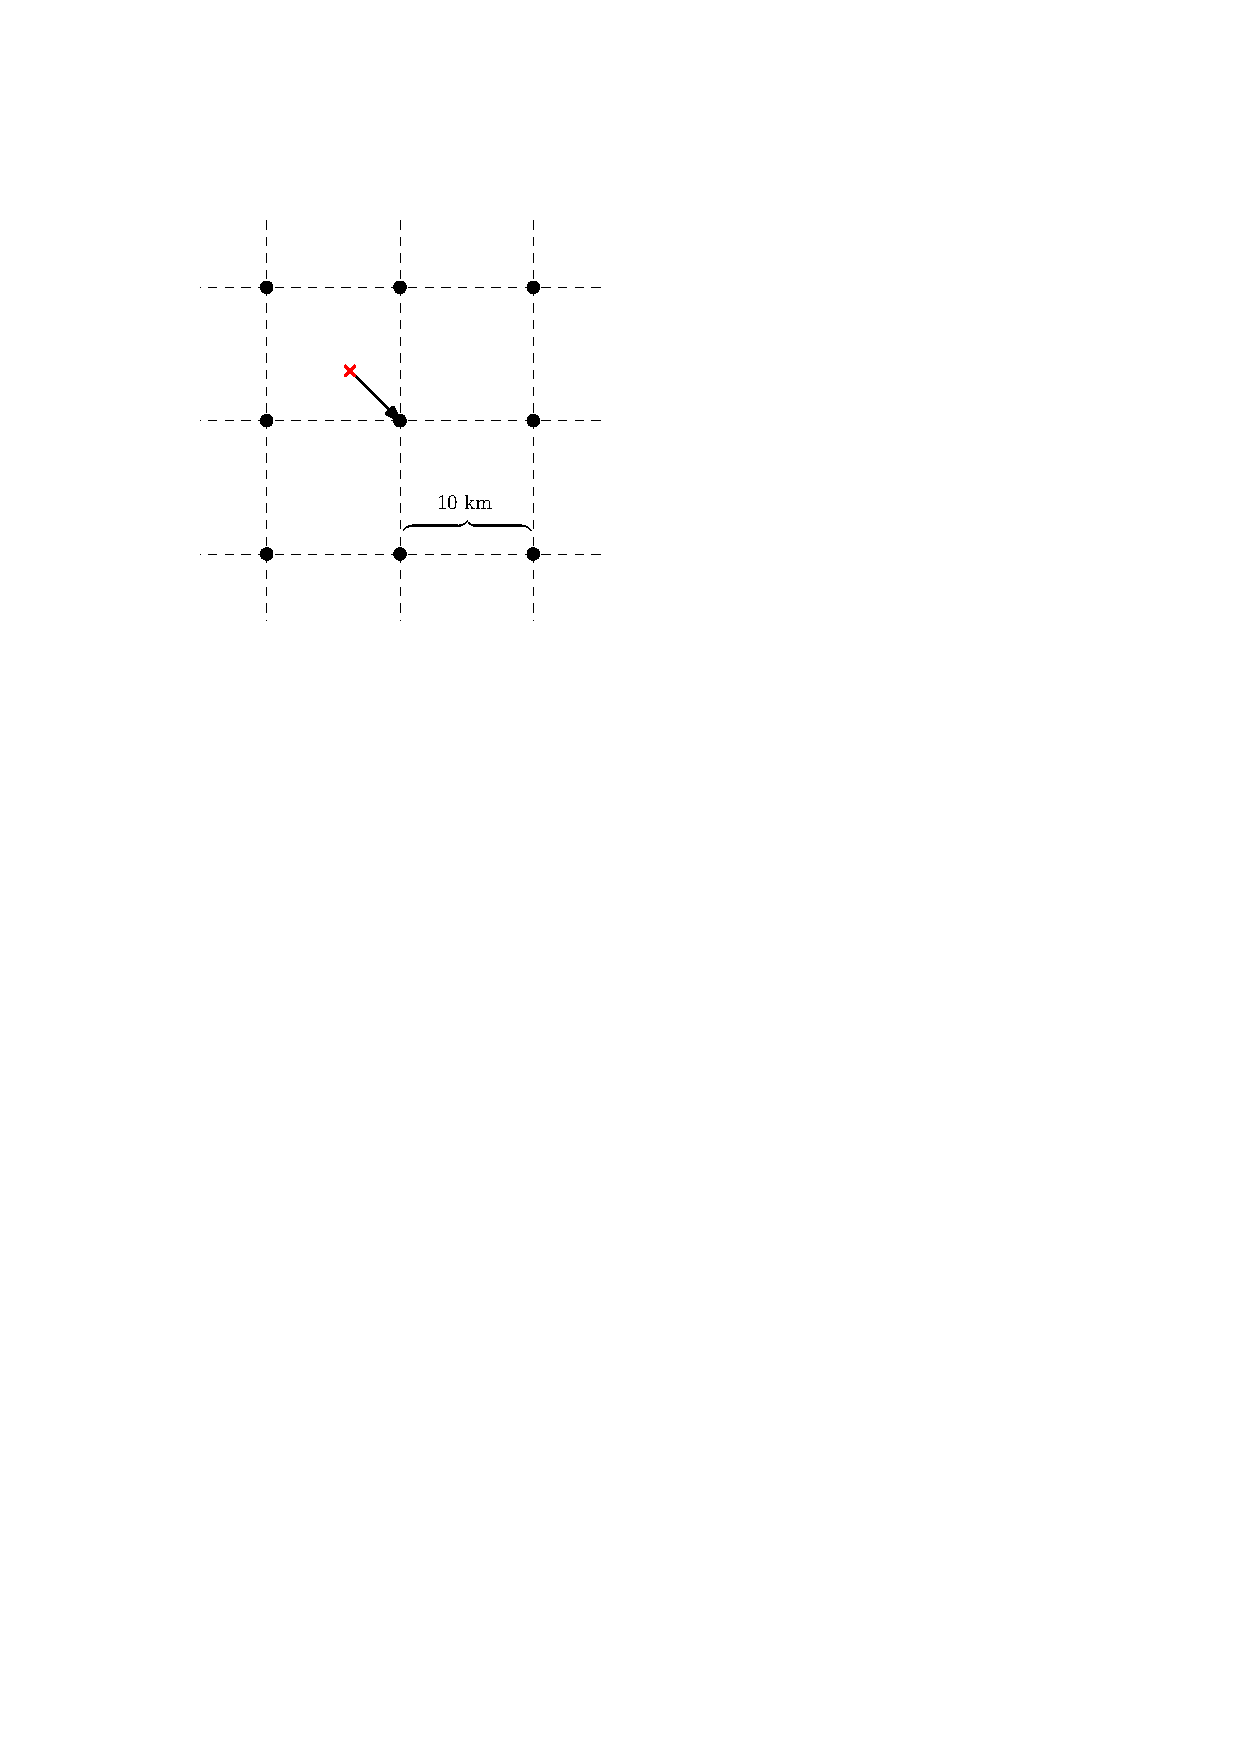
\includegraphics[width=.6\columnwidth]{location_grid_truncation_example}
  \caption{The user (represented by the red cross) has their location
    truncated to a grid of fixed points.}
  \label{fig:grid-truncation-example}
\end{figure}

Once we can intercept calls that pass location information to the app,
it is easy to modify the coordinates however we wish. As discussed
earlier, for our experiments, we truncate location information,
snapping to a user-specified grid, as illustrated in
Figure~\ref{fig:grid-truncation-example}.  Formally, our
implementation truncates to a grid with spacing $s$ in kilometers
using the formulae:

\begin{displaymath}
  \begin{array}{cc}
%    s_\textit{lat} = s \cdot \Delta^{\textit{lat}} &
    \textit{lat}' = s_\textit{lat} \lceil \textit{lat} /s_\textit{lat} \rceil &
%    s_\textit{long} = s \cdot \Delta^{\textit{long}} &
    \textit{long}' = s_\textit{long} \lceil \textit{long} /s_\textit{long} \rceil
  \end{array}
\end{displaymath}

\noindent where \textit{lat} and \textit{long} are the actual latitude and
longitude; their primed versions are the new coordinates. Here
$s_\textit{lat}$ and $s_\textit{long}$ are the grid spacing translated
into degrees of latitude and longitude, respectively.
%$\Delta^{loc}$ is number of degrees per meter, which differs for latitude and
%longitude.  
For latitude we use the approximation for North America \cite{latitude-calculator}:
\begin{displaymath}
s_\textit{lat} = \frac{s~\textrm{km}}{111.5~\textrm{km/deg}}
\end{displaymath}
%North America ($\Delta^{\mathit{lat}} \approxeq 111.5 \textrm{km}/\textrm{deg}$).
For longitude we use a standard approximation \cite{rapp:geometric}:

\[
s_\textit{long} = s~\textrm{km} \cdot 
  \frac {180 \sqrt{(1 - e^2 sin^2(\phi))}}
  {\pi a cos(\phi)}
\]

\noindent where $e^2 = (a^2 - b^2)/b^2$ is the eccentricity of Earth, $\phi$ is
the latitude, $a$ is the radius from the center of the earth to the
equator, and $b$ is the radius from the center of the earth to the poles.

We verified that \fuzzer{} works correctly in two ways.  First, we 
inserted logging code in \fuzzer{} to give the original position and 
position after location truncation.  We then took the set of locations from our 
testcases, truncated them to varying amounts, and then verified the
resulting positions were correct.  Second, we confirmed that our subject apps'
behaviors changed in sensible ways as we varied the location truncation 
amount.

The Android location
manager API also includes an option to report speed to apps, so our
implementation truncates speed using the same formula. However, none
of our subject apps use speed information. Moreover, device-reported
speed is often unreliable, so many apps ignore it, preferring
instead to estimate speed using successive location fixes.

\section{Experimental Design}
\label{sec:design}

\begin{figure}
  \small
  \begin{subfigure}{\columnwidth}
    \centering
    \begin{tabular}{|l|l|}
      \hline
      Name & Objects in List \\ \hline \hline
      \gasbuddy & Gas stations \\
      \restaurantfinder & Restaurants \\
      \hospitals & Hospitals \\
      \webmd & Pharmacies and clinics \\
      \walmart & Stores \\
      \tdbank & ATMs and branches \\
      \hline
    \end{tabular}
    \caption{Descriptions of each subject app.}
    \label{fig:app-descriptions}
  \end{subfigure}

  \bigskip{}

  \begin{subfigure}{\columnwidth}
      \centering
      \begin{tabular}{|l|r|r|}
        \hline
        City & Population & Radius (km) \\ \hline \hline
        New York, NY & 8,200,000 & 30 \\ \hline
        Dallas, TX & 1,200,000 & 20 \\ \hline
        New Haven, CT & 130,000 & 10 \\ \hline
        Baltimore, MD & 620,000 & 12 \\ \hline
        Redmond, WA & 54,000 & 4 \\ \hline
        Decatur, TX & 6,000 & 4 \\ \hline
      \end{tabular}
      \caption{Selected population centers.}
      \label{fig:regions}
    \end{subfigure}

    \bigskip{}

    \begin{subfigure}{\columnwidth}
      \centering
      \begin{tabular}{|r|r|r|r|r|} \hline
        0 km & 0.1 km & 0.2 km & 0.5 km & 1 km \\ \hline
         2 km & 5 km & 10 km & 20 km & 50 km \\ \hline
      \end{tabular}
      \caption{Truncation amounts tested.}
      \label{fig:truncations}
    \end{subfigure}

  \caption{Experimental parameters.}
\end{figure}
 
We conducted a systematic study of the effect of location truncation
on apps that list nearby objects (the largest category of apps in
Figure~\ref{fig:location-uses} in which location truncation's effect is clearly
measurable). We selected a variety of such apps, listed in
Figure~\ref{fig:app-descriptions}, from Google Play. We chose apps
that rely on a variety of different data sets and ran under our tool
chain with minimal difficulty.
We then modified each app using \fuzzer, as outlined
in Section~\ref{sec:impl}. Next, we randomly chose a set of locations and
then captured the output list of each app as we varied the current
location and the amount of truncation applied to it. Finally, we used
several metrics to estimate how each truncation affected the app's
utility.

\subsection{Locations and truncations}

In a pilot study, in which we examined the results of \fuzzer{} on a
variety of apps, locations, and truncations in an ad hoc manner,
we noticed that truncation has quite different
effects depending not only on the app, but also on where the app is
run. For example, there is a significantly higher density of restaurants in
a big city than in a rural area, causing one of our subject apps,
Restaurant Finder, to behave very differently under truncation in each locale.
Thus, in selecting locations for
our study, we chose them from a range of population centers of varying
sizes, as shown in Figure~\ref{fig:regions}. 

We modeled each city as a circle centered on the geographical 
city center with a radius estimated
from looking at a map of the region. In
our pilot study, we also found that many apps produce error screens if
given a location that cannot be mapped to a real address, e.g., if the
current location is in the ocean or a heavily forested area.
Thus, we discarded any random points that caused 
problematic outputs from our apps, and randomly picked new
points until we had a set of 10 points that produced correct output
across all apps when the apps were run with no truncation.

For each random location, we ran each app with 10 different truncation
amounts, including no truncation, listed in
Figure~\ref{fig:truncations}.  We chose an upper limit of 50 km because 
many apps in our 
test set only give results up to or less than 50 km, so the metrics would
be undefined if we went beyond that level of truncation.

\subsection{Metrics used for evaluation}
\label{sec:metrics}

Recall from Section~\ref{sec:usage} that we identified apps that list
nearby objects as the best candidate for our study of location
truncation. For example, Figure~\ref{fig:app-example} gives two
screenshots of the Restaurant Finder app being run on a location in
New York, NY (close to Bloomfield, NJ) both without and with
truncation. Here the lists we consider are the restaurants, in order
from closest to farthest, along with their distances.

We explored three different ways to measure location truncation's effect on
the output list of such apps: edit distance of the changed list from the
original, the size of the intersection of the original and changed
lists, and the additional distance of the first (closest) list item on
the changed list.

\begin{figure}
  \centering
  \begin{tabular}{cc}
    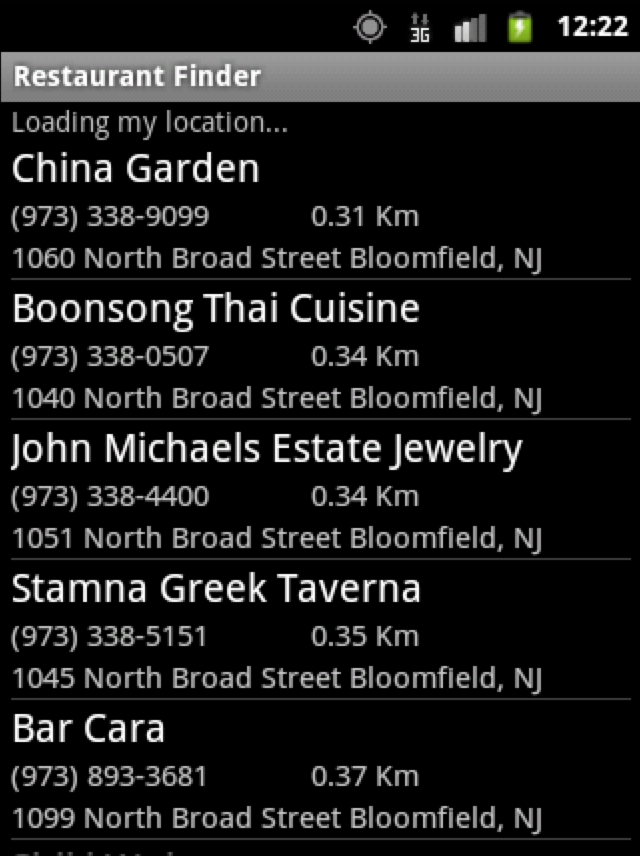
\includegraphics[width=.4\columnwidth]{restaurant_finder_ref_screenshot}
    & 
    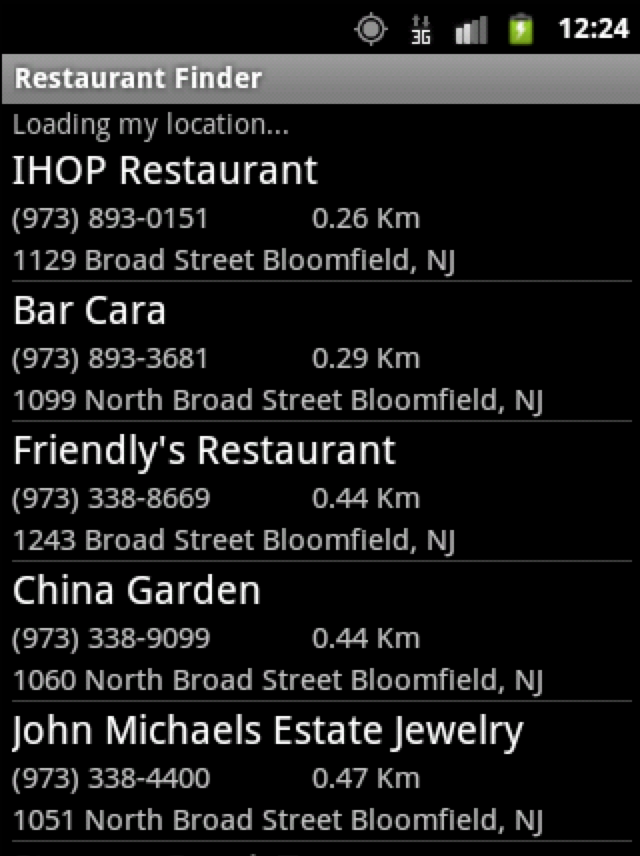
\includegraphics[width=.4\columnwidth]{restaurant_finder_nominal_screenshot}
  \end{tabular}
  \caption{Restaurant Finder without (left) and with (right)
    0.2~km of truncation.}
  \label{fig:app-example}
\end{figure}

\paragraph*{Edit distance}

The first metric we investigated is \emph{edit distance}, which is the
number of edits needed to change one list into another. This is the
traditional Levenshtein distance \cite{levenshtein:1966}, in which an
edit is an insertion, deletion, or swap of two list elements. For
example, the edit distance between the lists in
Figure~\ref{fig:app-example} is five, because every item in the
list has changed.

Like the other apps we studied, Restaurant Finder returns more than
one screenful of objects. Thus, in performing our measurements, we
need to decide how much of the app's output to use. We could pick only
the first screen of data, but this restricts edit distance to just
a few possible values. We could pick all the results, but that has the
disadvantage that there could be many changes in the long tail of a
list, yet few users would bother looking that far. Thus, as a
compromise, we opted to compute edit distance over the first four
screens of an app, which we think covers typical usage patterns while
providing useful data.  In each of the apps we tested, this corresponded 
to the first twenty elements of the list.

\paragraph*{Set intersection size}

Edit distance was the first metric we thought of, but when we tried
measuring it (Section~\ref{sec:results}) we found it to be
problematic: Especially on the first screen of data, many locations
are very close together, e.g., on the left of
Figure~\ref{fig:app-example}, distances range from 0.31~km to
0.37~km. Yet edit distance would count reorderings of those locations
in the metric.

Thus, we also explored using set intersection size as a metric. We
ignore ordering and compute how many objects are in both the original
and changed list; the higher the number, the more similar the
lists. For example, in Figure~\ref{fig:app-example}, the set
intersection has size three. As with edit distance, we compute the
intersection on the list displayed across the first four screens of
output.

The set intersection metric is also more natural than edit distance in
that it corresponds directly to a common user task of checking whether
some particular object is nearby, e.g., we might use Restaurant Finder
to ask, is there any McDonalds nearby, or we might use GasBuddy to
look for the closest Shell station.

\paragraph*{Additional distance incurred}

Ideally, we would like to measure how actual users' behavior is
affected by location truncation, but this is difficult to do without a large
number of human participants. Instead, we developed an \emph{additional
  distance} metric that computes how much farther a user who always
picks the first list item would go given the changed list compared to
the original list.

For example, in Figure~\ref{fig:app-example}, the closest restaurant
is actually China Garden, 0.31 km away. However, under truncation, the
closest restaurant appears to be an IHOP. While the IHOP's reported
distance is 0.26 km, that is the result from the truncated
location---we need to look at the original output list to find out how
far away the restaurant actually is. In this case, IHOP appears on the
second screen of the original list, and it is 0.42~km
away. For this example, then, the additional distance is $0.42 - 0.31
= 0.11$~km.

%%\jeff{Talk about the number of screens looked at.}

Restating this more generally, let $D(X)$ be the distance to object
$X$ on the original list. Then the additional distance of a changed
list is $\Delta = D(\textit{First original}) - D(\textit{First changed})$, where
\textit{First original} is the first item of the original list and
\textit{First changed} is the first item of the changed list. Notice
that this metric may be undefined if \emph{First changed} does not
appear on the original list. To reduce the chances of this, we
consider all output screens of an app in computing the metric, and not
just the first four screens. However, in our experiments the metric is
still sometimes undefined for some apps under large truncation amounts.

\subsection{Testing infrastructure}

To compute the results of our experiments, we needed to run each
subject app at each of 60 locations and 10 different truncation
amounts. This is clearly far too many configurations to run by
hand. Instead, we developed testing infrastructure to let us run each
configuration automatically, scrape the resulting output lists, and
then run our metrics on the result.

The core technology we used is Troyd \cite{jsjeon:troyd}, an open source,
black box testing framework that can execute apps (e.g., launch them,
click buttons, enter text boxes, scroll the screen, etc.) and gather
text from the GUI. 
Troyd allows us to write a high level test case (e.g., to click a sequence of
buttons and gather some text) that can be reused for various test 
configurations.
We developed a server that takes an app modified by
\fuzzer{}; resigns it with a shared user ID so that it
can be controlled by instrumentation; and then runs testcases against
the app using Troyd.

We ran apps on both actual mobile phones (Google Nexus S devices) and
device emulators; our infrastructure works the same in both cases, and
performing some runs on actual devices acted as a sanity check. In all
cases, the Android platform was Gingerbread 2.3.3 with the Google
APIs installed. These APIs are special dynamic libraries licensed by Google and not included 
on vanilla Android distributions, such as maps,
installed on the device or emulator; these APIs are
needed for the subject programs to run.

We found that, while Troyd mostly did what we wanted, we needed to
extend it to handle additional GUI elements.
For example, while Troyd can capture the currently visible GUI elements,
many \code{Views} (such as those in \code{ListView} elements) are 
reused and their contents only appear when the screen is scrolled.
This meant Troyd had to expose certain elements to ensure these were 
rendered.  To do so, we extended Troyd with special functionality to 
navigate to screens that may have unrendered information.
We also found that, as is usual in large-scale
testing, we needed our infrastructure to handle failure. In some cases,
experimental tests failed unpredictably, e.g., an emulator
or device would crash for no apparent reason. These are likely due to
subtle bugs lurking in the OS or in the emulator implementation that
were tickled by the experiment's atypical usage pattern. Thus, our
testing infrastructure catches any failed runs and reschedules those
experiments to be run again. Finally, our testing infrastructure allows
multiple experiments to be done in parallel; the majority of the
experiments were done on a machine with six Intel Xeon processors, 
each with four cores, and 48 GB of RAM.  Our tests ran up to fifteen
emulators at once.

% The script first clicks through a set of screens in the app which
% request if the user wants to register for an account, and then selects
% a screen to get a list of gas stations near the user.  Once the screen
% is presented, we retrieve the list of GUI elements from the app and
% then dump them to a file for post processing.

\begin{figure*}[t!]
  \centering
  \begin{tabular}{ccc}
    
    \begin{minipage}{2in}
      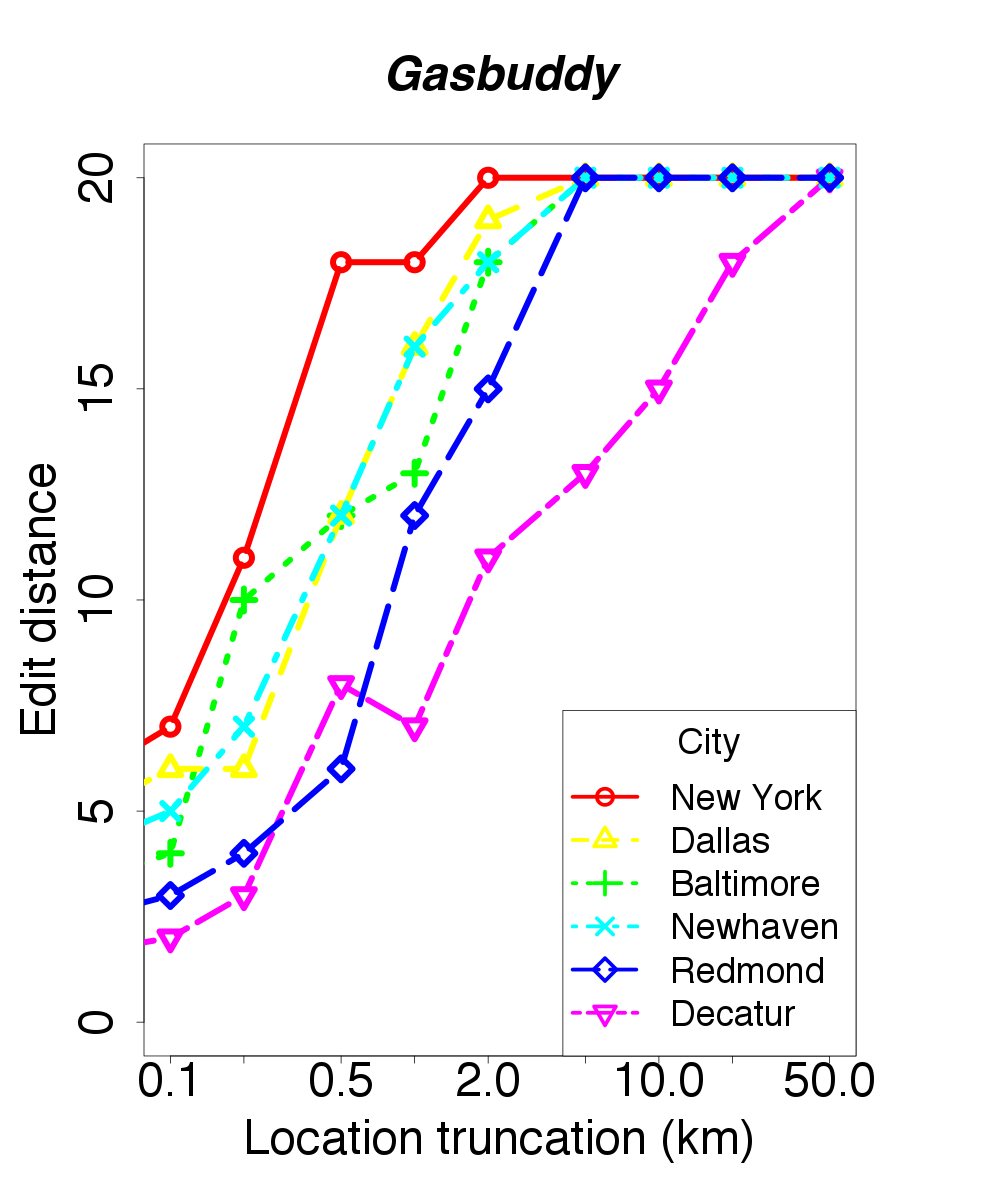
\includegraphics[width=\textwidth]
                      {data/gasbuddy/plots/medians_across_city_20}
    \end{minipage}
    
    % [width=.6\textwidth]
    \begin{minipage}{2in}
      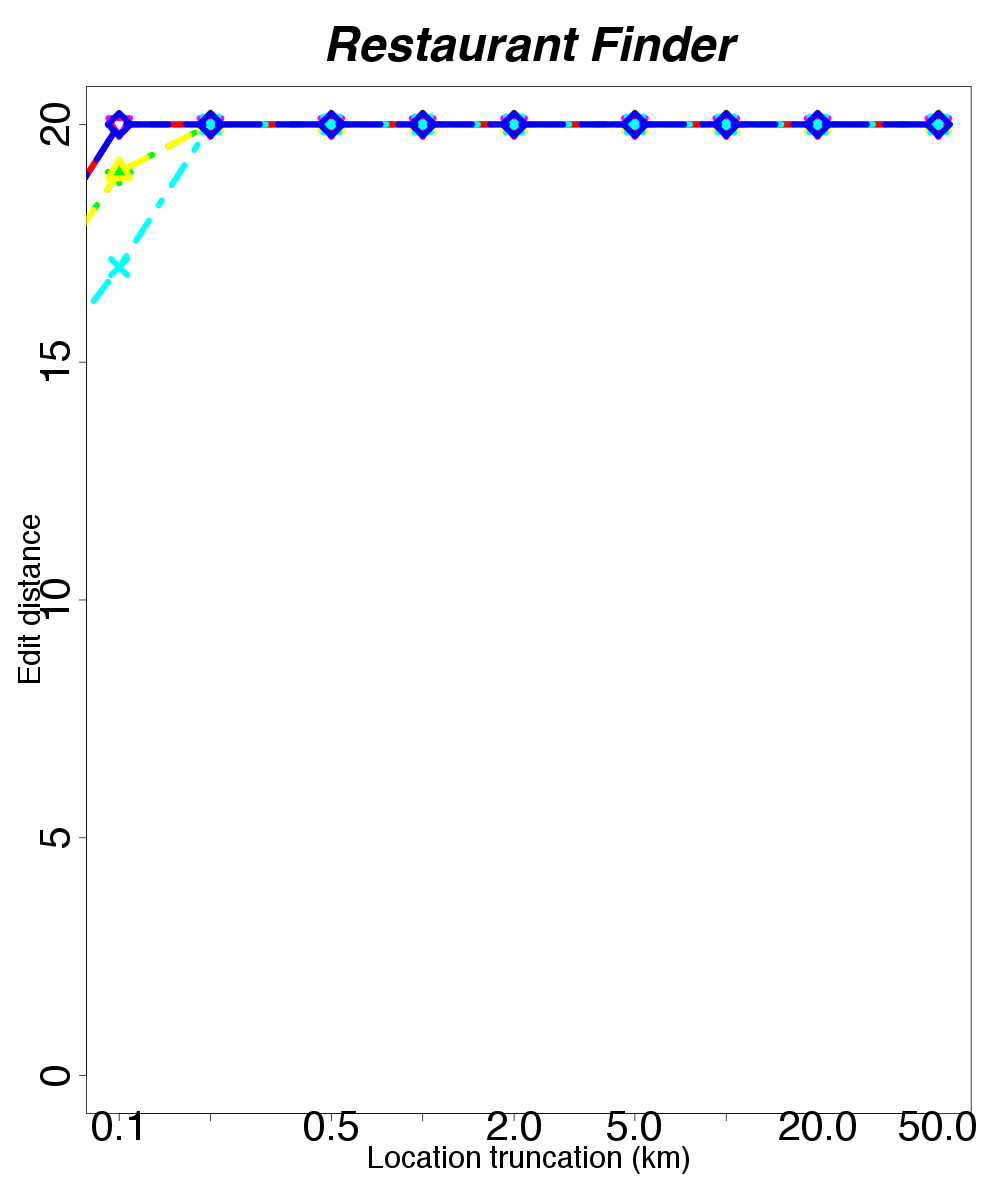
\includegraphics[width=\textwidth]
                      {data/restaurant_finder/plots/medians_across_city_20}
    \end{minipage}
    
    \begin{minipage}{2in}
      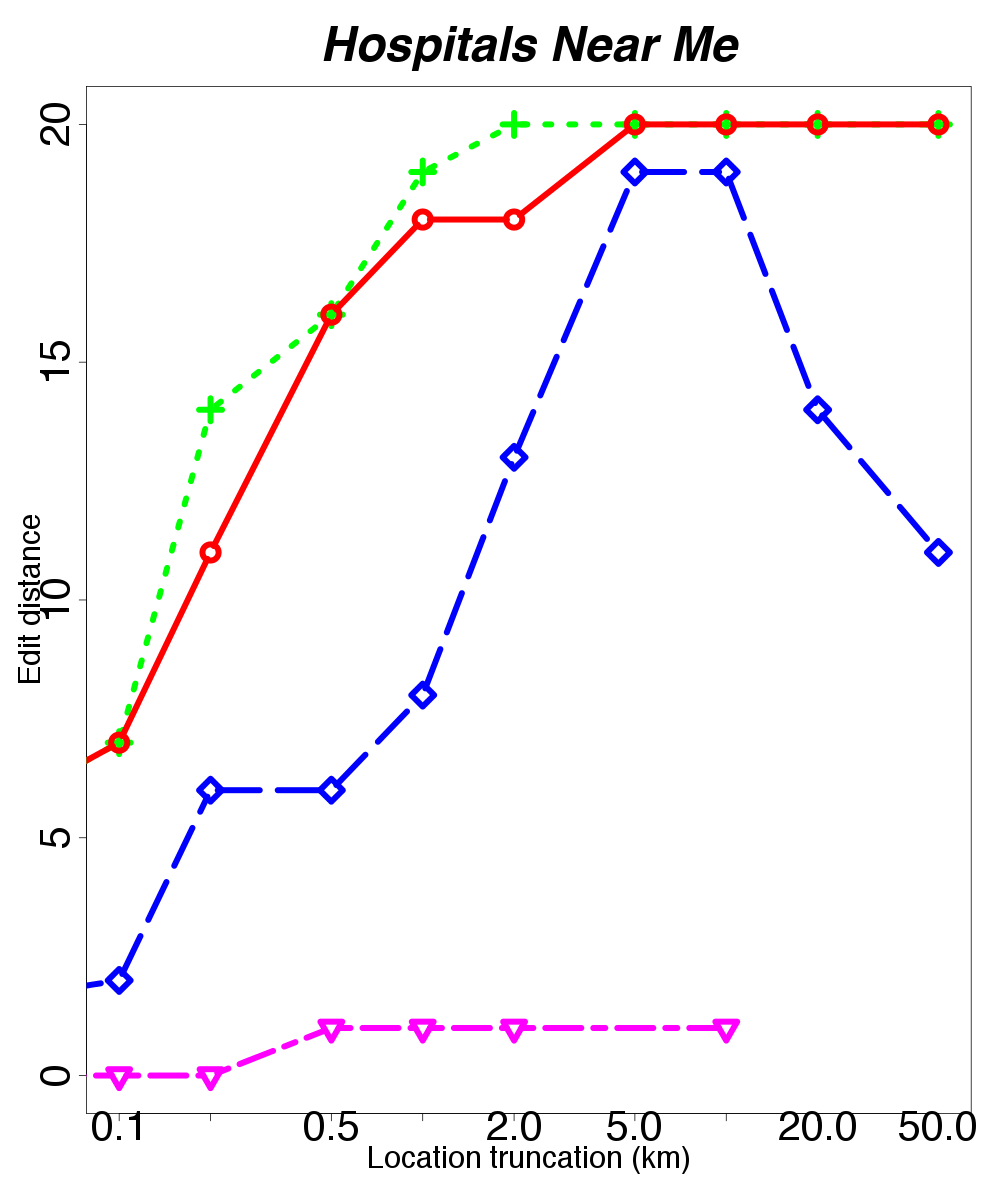
\includegraphics[width=\textwidth]
                      {data/hospitals/plots/medians_across_city_20}
    \end{minipage}
    
    \\
    \begin{minipage}{2in}
      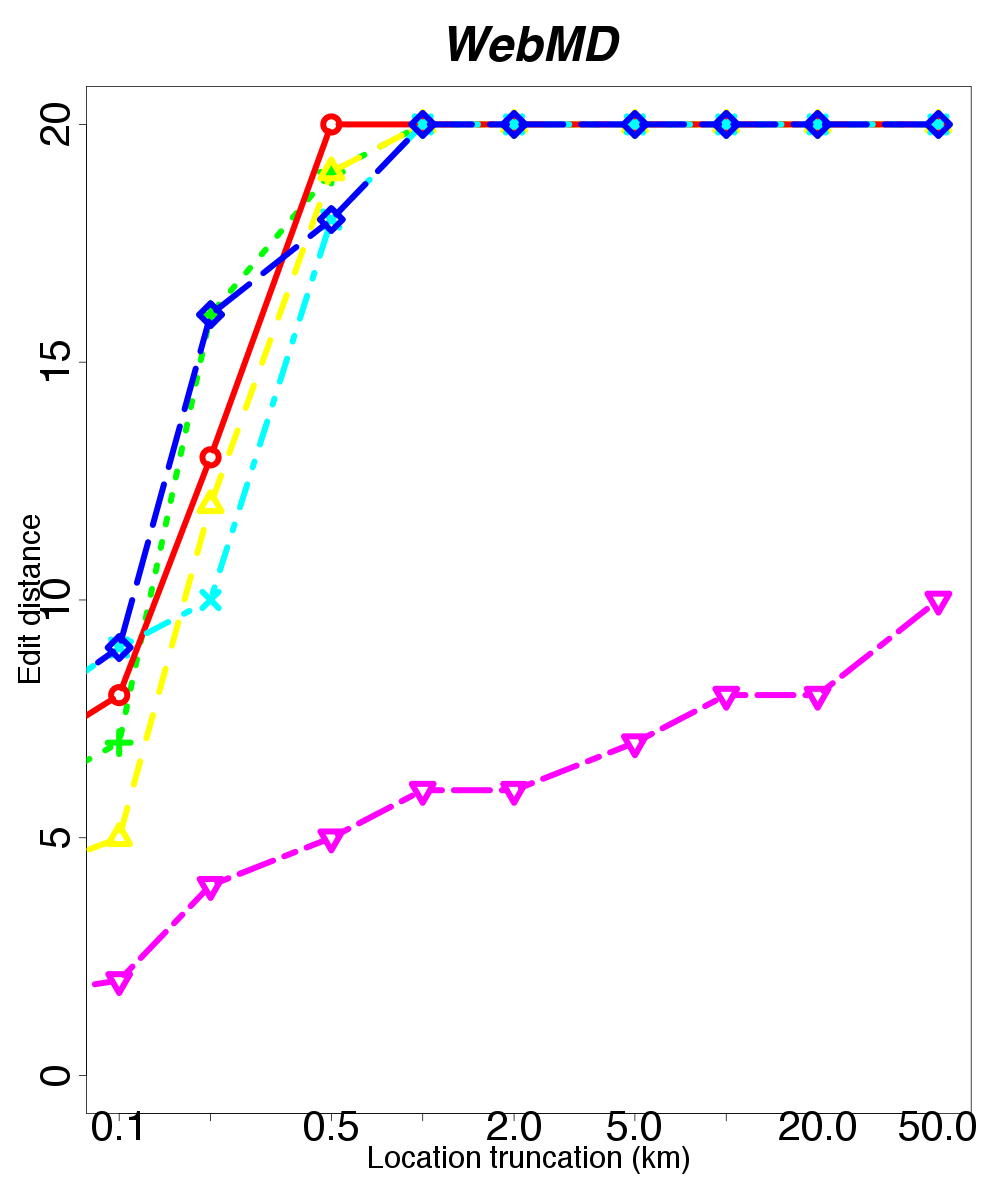
\includegraphics[width=\textwidth]
                      {data/webmd/plots/medians_across_city_20}
    \end{minipage}
    
    \begin{minipage}{2in}
      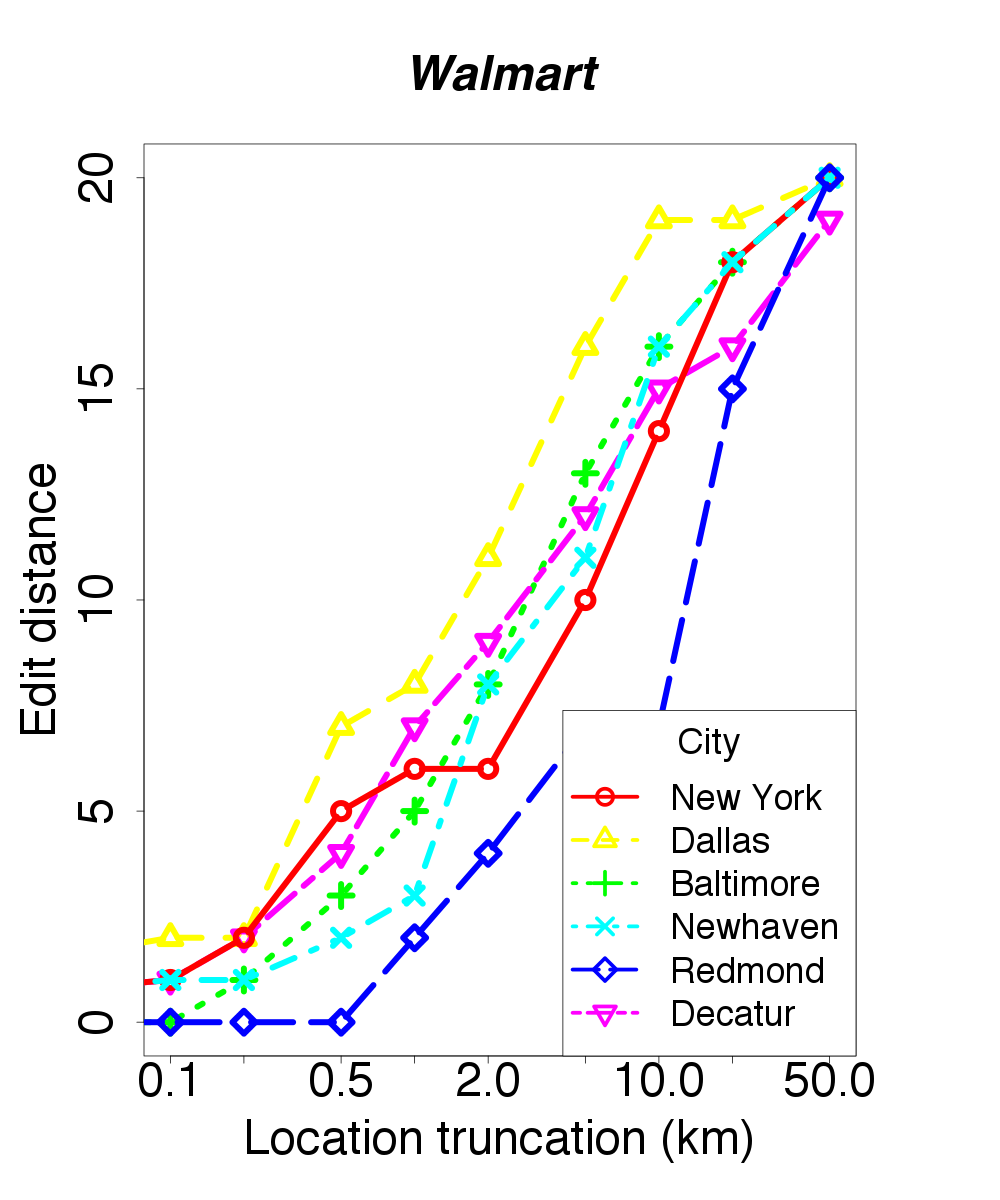
\includegraphics[width=\textwidth]
                      {data/walmart/plots/medians_across_city_20}
    \end{minipage}
    
    \begin{minipage}{2in}
      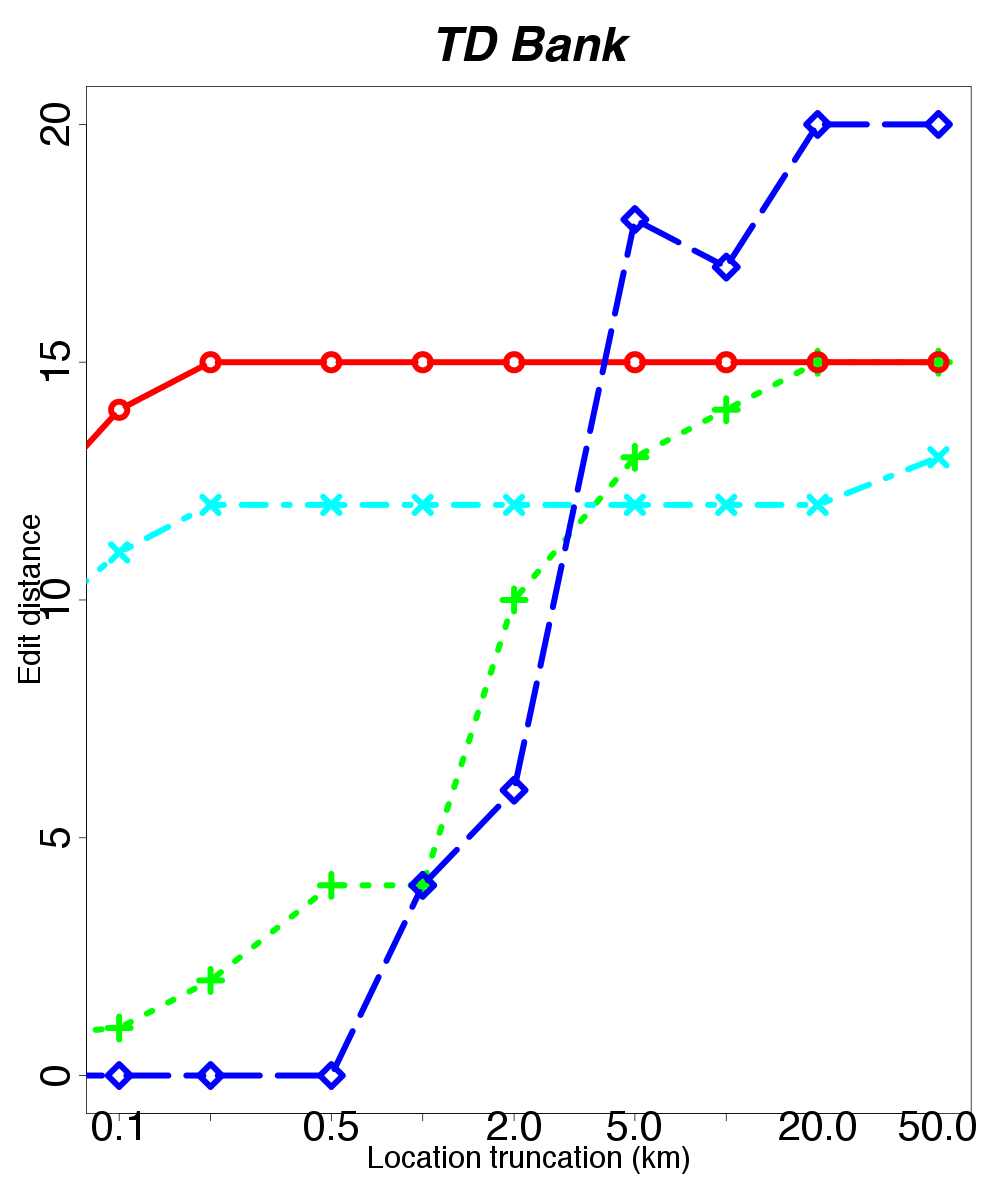
\includegraphics[width=\textwidth]
                      {data/tdbank/plots/medians_across_city_20}
    \end{minipage}
  \end{tabular}
  \caption{Graphs of median edit distance versus truncation
    amount. Higher edit distance implies lower utility.}
  \label{fig:edit-distance-metric}
\end{figure*}

\section{Results}
\label{sec:results}

Across our
subject apps and locations, we found that location can be
significantly truncated without significantly harming utility: up to 20~km
when an app is used in a lower population area, and usually (for five of six apps) 
at least 5~km in more populous areas.  We also found that apps have relatively little 
change in utility up to a certain amount of truncation, typically
about 5~km, after 
which the app's output becomes much less usable.  Finally, we found that the factor 
that most determines the ability to truncate location was the density
of the set of locations the app computes over (hospitals, gas stations, etc...).

In the discussion that follows, we include several plots. In each
plot, the x-axis is the truncation amount; note that because of our
choice of truncations, this axis is essentially log-scale.  The y-axis
is the median of one of our metrics on the 10 randomly chosen points
for each population center.

% Also note that the truncation amounts are an upper bound of 
% how much the location changes, e.g., if a location is on a grid point,
% then truncating it has no effect. 
% Because of this, we took the median of ten randomly 
% selected points.
% The y-axis is the utility, the interpretation of which varies by metric.

% We also study where apps degrade past a usable quality of output (this
% is taken as a parameter in \cite{Shokri:2012}, for example).  For each
% metric we define an acceptable cutoff of usable output based on utility.
% We fix this cutoff for each metric and investigate --- for each app --- how 
% this metric varies.

%% For each trend line, we compute the \emph{inflection point} at which
%% utility changes the most using the \emph{maximum finite difference}. 
%% For a sequence of points $(x_i,y_i)$, we define the finite difference of 
%% a point as

%% \begin{figure}[h]
%% \begin{center}
%% \[
%% \mathit{fdiff}(x_{i},y_{i}) = 
%% \frac{\frac{y_{i+1}-y_{i}}{2 (x_{i+1}-x_{i})} 
%%   - \frac{y_{i}-y_{i-1}}{2 (x_{i}-x_{i-1})}}
%%      {x_{i+1}-x_{i-1}}
%% \]
%% \end{center}
%% \end{figure}

%% Then the inflection point is the $i$ such that $\cdiff(y_i)$ is
%% maximized.

%%
%% Figure for additional distance metric.
%%

We next consider each of our three metrics (discussed in Section~\ref{sec:metrics})
in turn.

\subsection{Edit Distance}

\begin{figure*}
  \centering

  \begin{subfigure}{\textwidth}
  \begin{tabular}{ccc}
    
    \begin{minipage}{2in}
      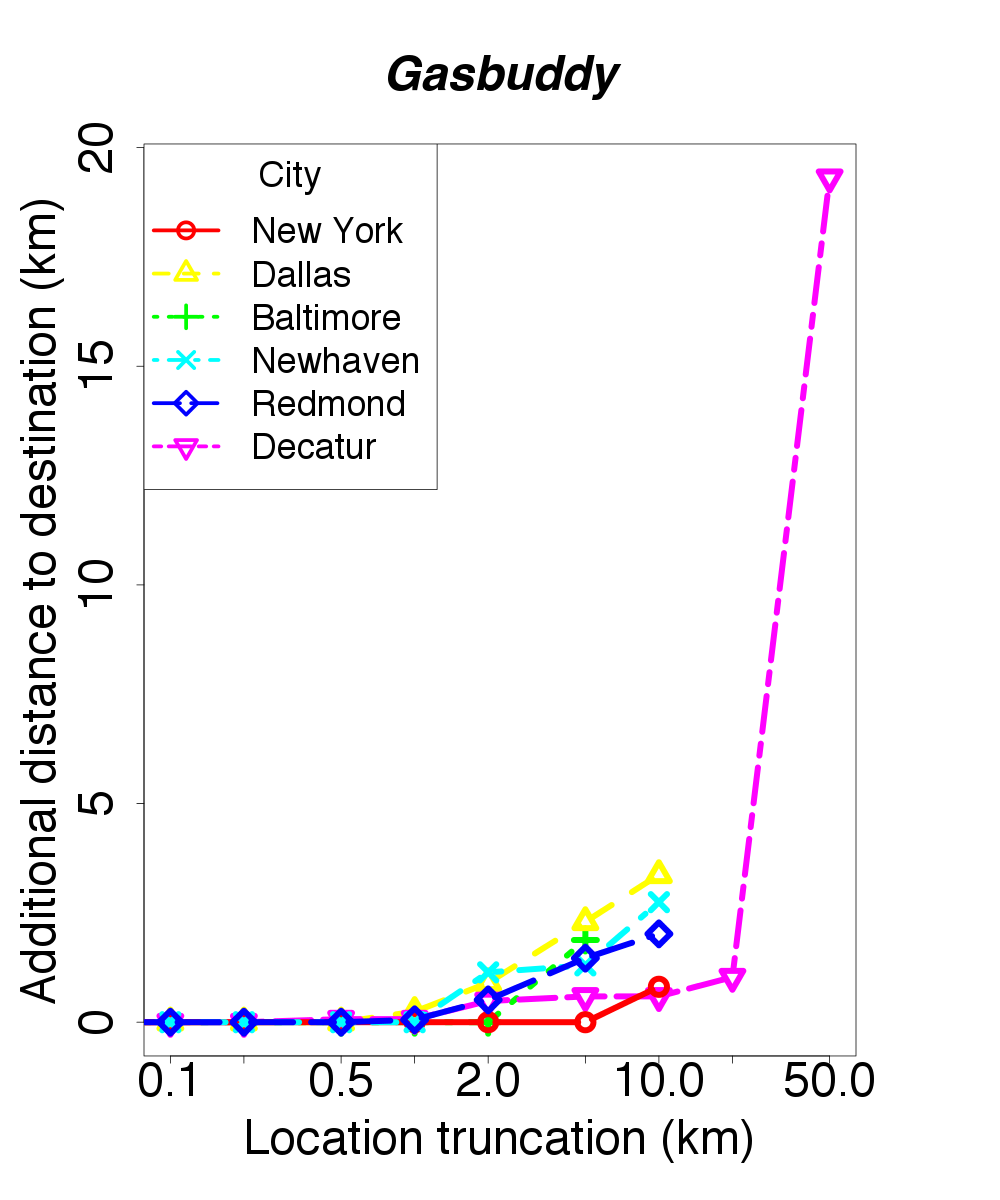
\includegraphics[width=\textwidth]
                      {data/gasbuddy/plots/medians_across_city_additional_distance}
    \end{minipage}
    
    % [width=.6\textwidth]
    \begin{minipage}{2in}
      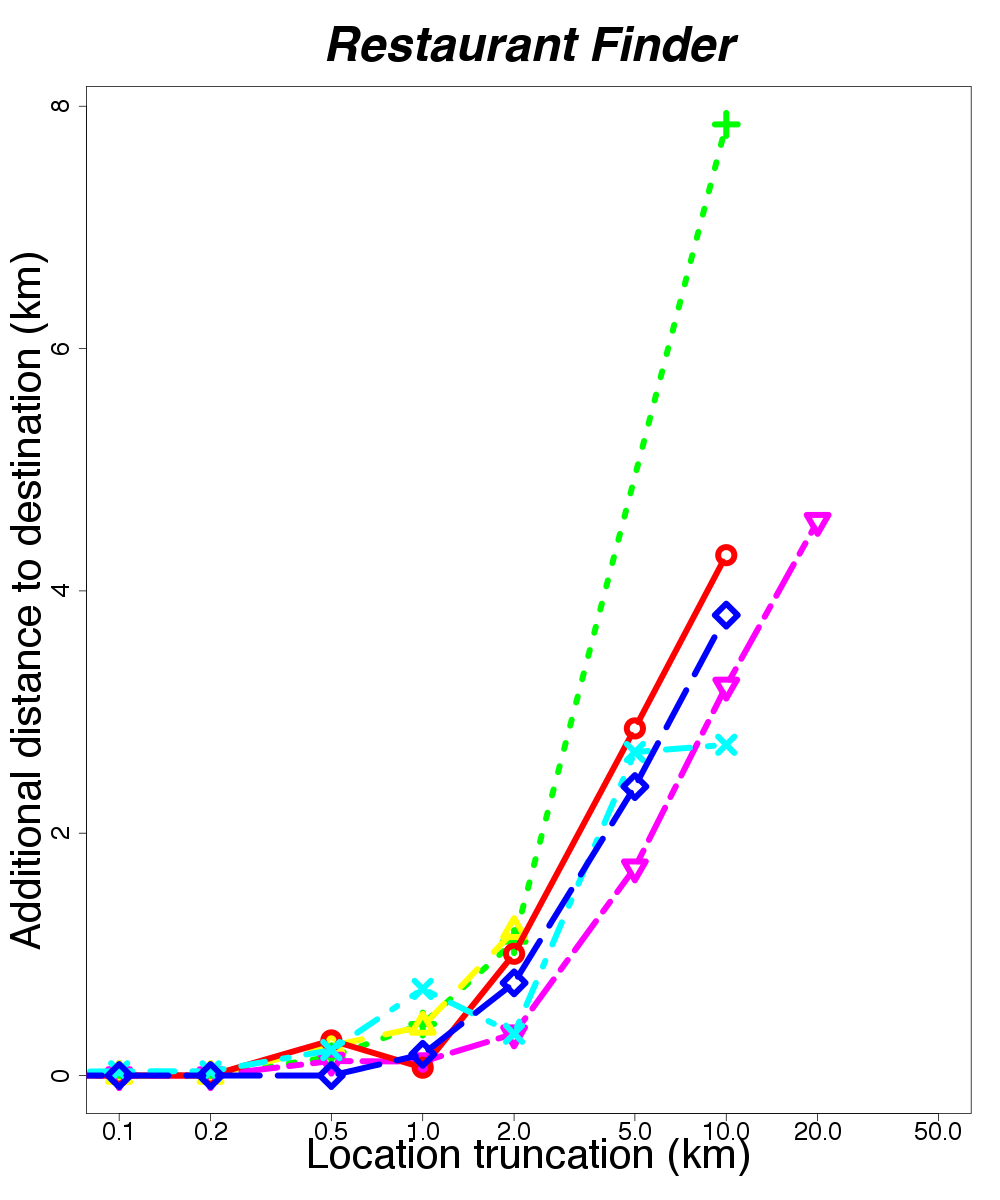
\includegraphics[width=\textwidth]
                      {data/restaurant_finder/plots/medians_across_city_additional_distance}
    \end{minipage}
    
    \begin{minipage}{2in}
      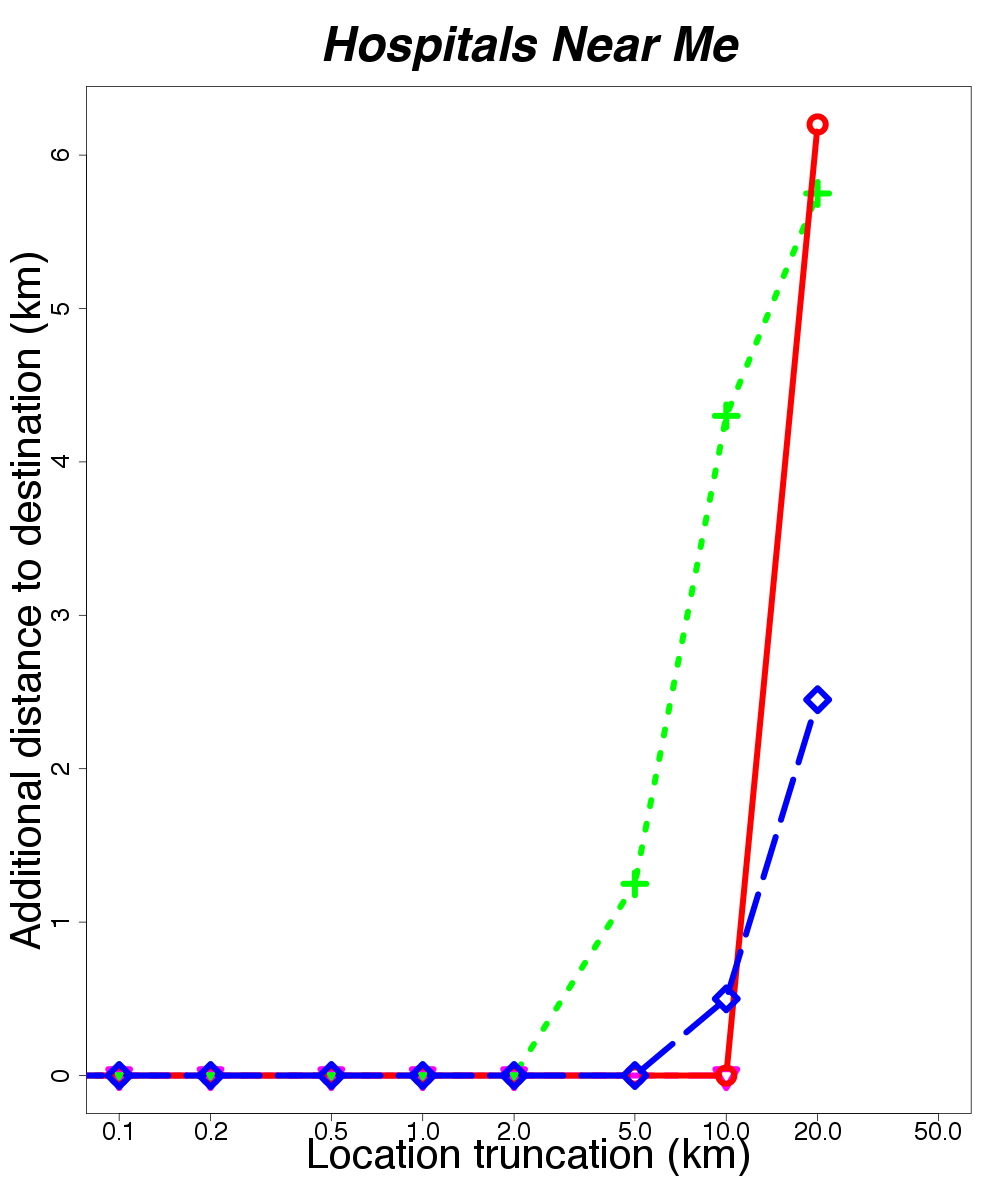
\includegraphics[width=\textwidth]
                      {data/hospitals/plots/medians_across_city_additional_distance}
    \end{minipage}
    
    \\
    \begin{minipage}{2in}
      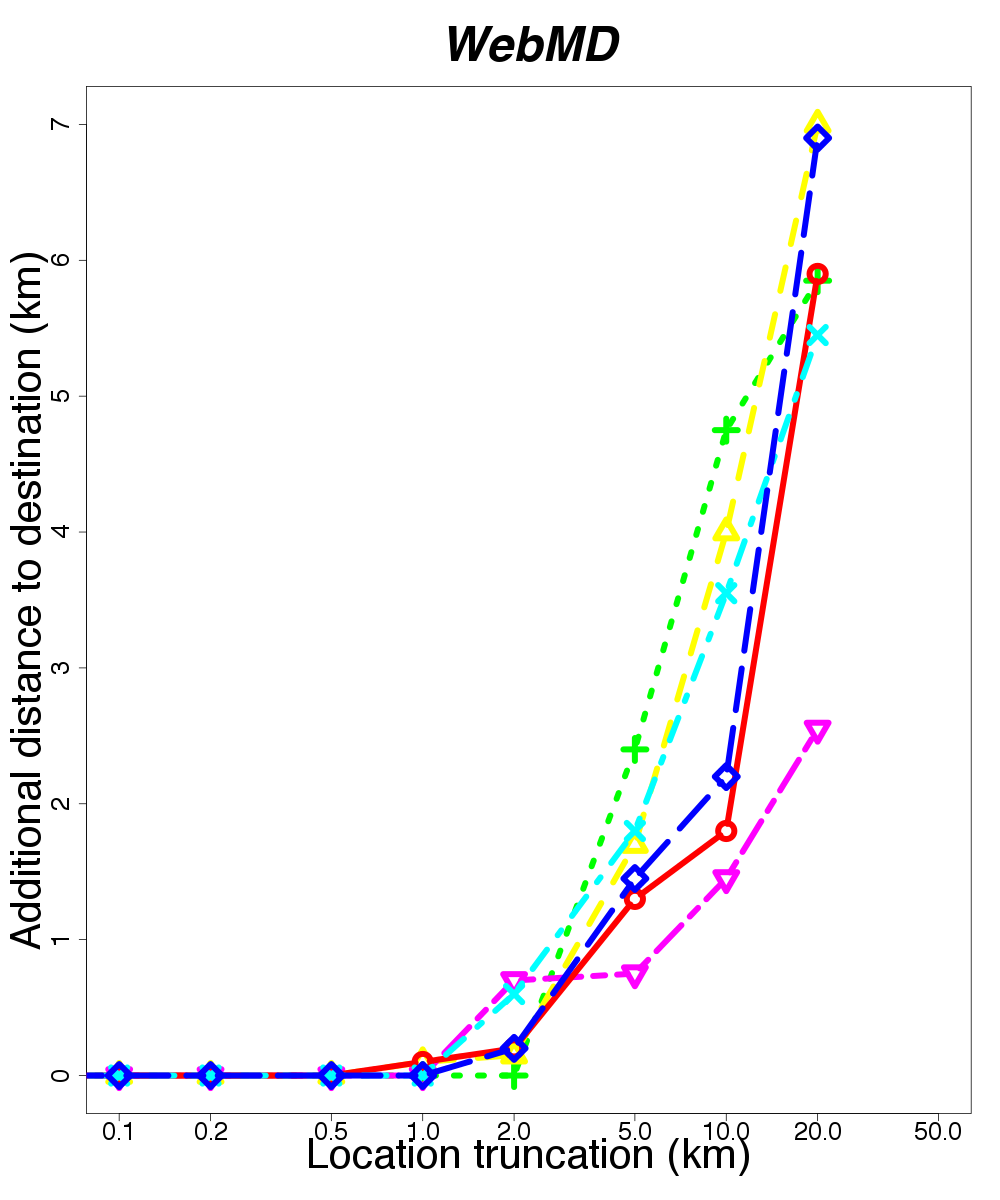
\includegraphics[width=\textwidth]
                      {data/webmd/plots/medians_across_city_additional_distance}
    \end{minipage}
    
    \begin{minipage}{2in}
      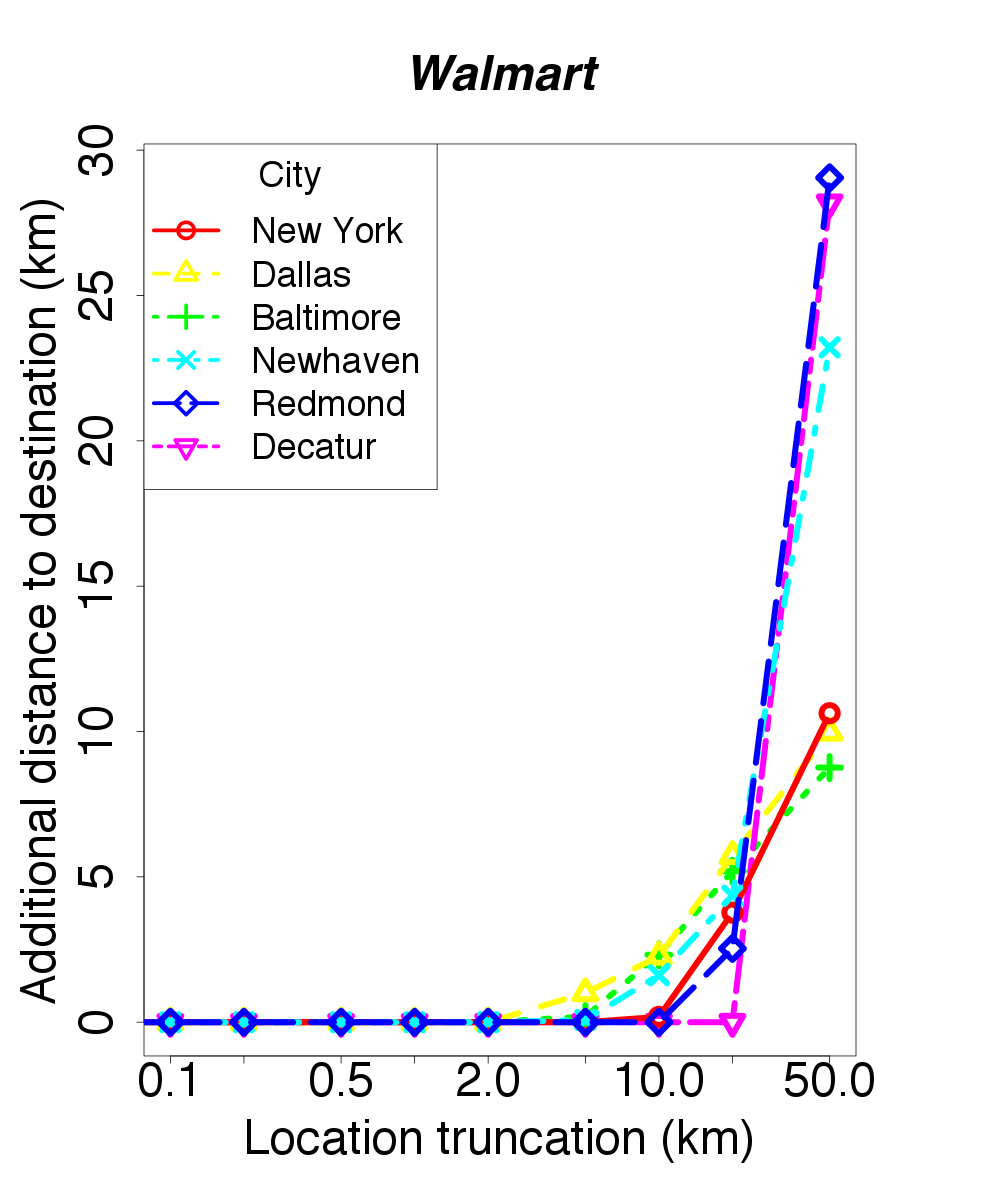
\includegraphics[width=\textwidth]
                      {data/walmart/plots/medians_across_city_additional_distance}
    \end{minipage}
    
    \begin{minipage}{2in}
      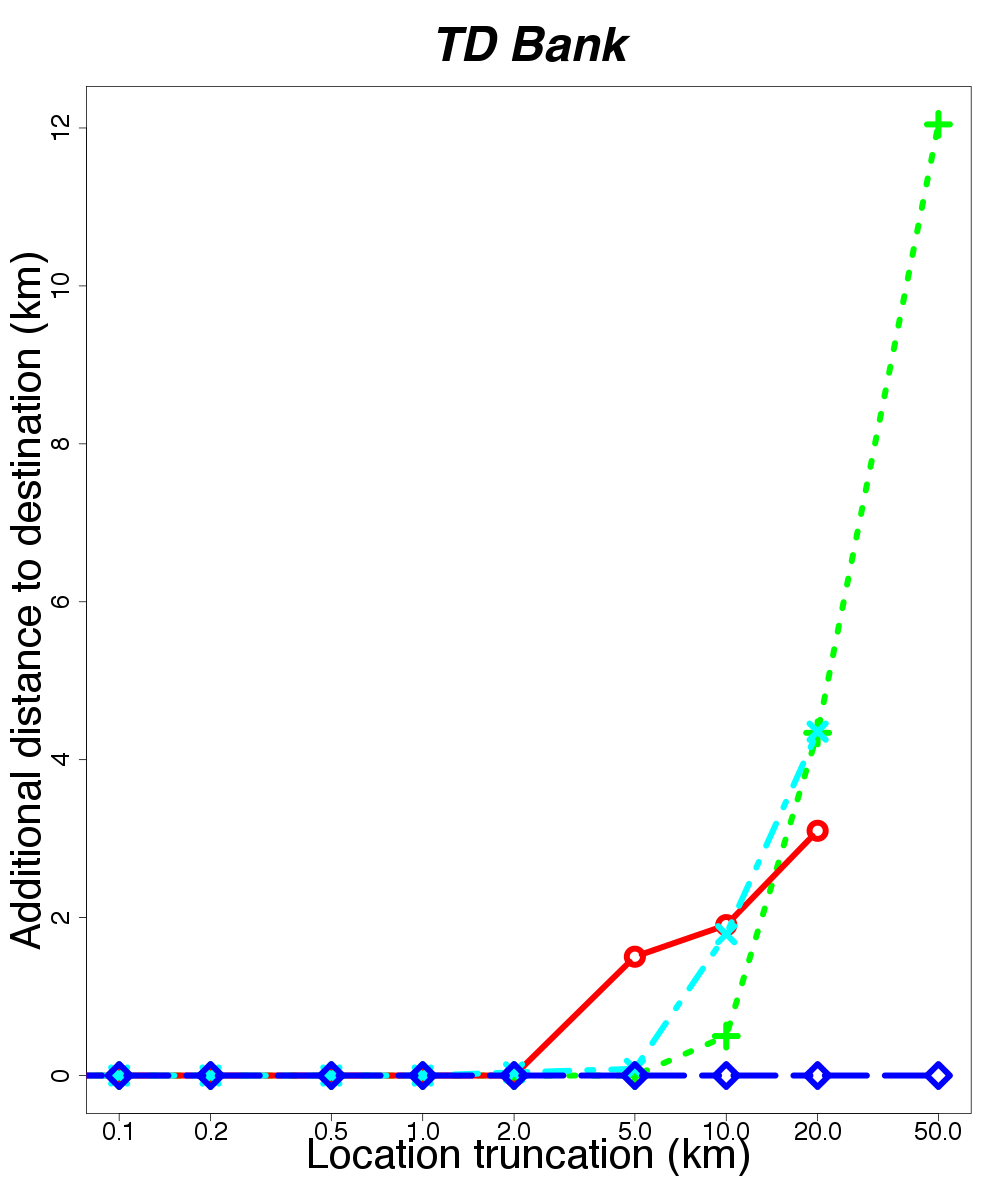
\includegraphics[width=\textwidth]
                      {data/tdbank/plots/medians_across_city_additional_distance}
    \end{minipage}
  \end{tabular}
  \caption{Graph of median additional distance versus
    truncation amount.  Higher additional distance implies lower
    utility.}
  \label{fig:add_distance}
  \end{subfigure}

  \bigskip{}

  \begin{subfigure}{\textwidth}
 \small
 \centering
 \begin{tabular}{|l||r|r|r|r|r|r|}
 \hline
 & New York & Dallas & Baltimore & New Haven & Redmond & Decatur \\
 \hline
 \hline
 Gasbuddy & $\cdot$ & 5 & 5 & 2 & 5 & 20 \\
\hline
Restaurant Finder & 2 & 2 & 2 & 5 & 5 & 5 \\
\hline
Walmart & 20 & 5 & 10 & 10 & 20 & 50 \\
\hline
TD Bank & 5 & $\cdot$ & 20 & 10 & $\cdot$ & $\cdot$ \\
\hline
WebMD & 5 & 5 & 5 & 5 & 5 & 10 \\
\hline
Hospitals Near Me & 20 & $\cdot$ & 5 & $\cdot$ & 20 & $\cdot$ \\
\hline

\end{tabular}
\caption{Largest truncation amount (km) before median additional
  distance exceeds 1~km.}
 \label{fig:knee-points-additional-cutoff}

  \end{subfigure}

\caption{Additional distance results.}
  
\end{figure*}
 
Figure~\ref{fig:edit-distance-metric} shows how edit distance 
 varies
on our location set.  
Note that Hospitals Near Me and TD Bank do
not have data for some cities because the app did not generate enough output
to calculate a significant result for those cities.  
For example, there are no TD banks in Dallas.  In some cases the two apps 
(TD Bank and Hospitlals Near Me) do generate data, but they generate 
a smaller list of apps.  This is why the edit distance appears to go down
at large truncation values for these apps: because in less populous 
locations they output smaller set of locations.

The plots show that in most cases, the output lists change to some
degree even at the smallest truncation level. Moreover, in two cases
(Gasbuddy and Restaurant Finder), the edit distance quickly reaches
its maximum value (all items in the list change) in several
locales. WebMD is similar, though it plateaus somehwat later. The
remaining three apps, in contrast, show a generally steady progression
of edit distance versus truncation amount.

The reason for these trends is density of objects--Gasbuddy,
Restaurant Finder, and WebMD all return lists of items that can
commonly be found everywhere, whereas there may be only a few
hospitals, Walmarts, or TD Bank locations. Indeed, looking at
Gasbuddy, we see that edit distance plateaus quickest for New York,
the most populous locale, and slowest for Decatur, the least populous
locale.

% approach the maximum value with very little truncation (these apps
% cannot be truncated more than 500 meters).  However, apps measuring
% less densely distributed objects (such as the \hospitals and
% \walmart apps) can have their inputs truncated to a much greater
% degree.  For edit distance, a maximum value means that no part of
% the nominal list is in the order of the reference list.  The three
% apps (\gasbuddy, \restaurantfinder, and \webmd) measuring dense
% locations quickly hit this maximum.  By contrast, apps measuring
% less densely distributed locations (\hospitals, \walmart, \tdbank)
% only reach this maximum value with large (50 kilometers for each
% case) amounts of truncation.

% Because apps almost universally base their measurements
% around euclidean distance on a two dimensional plane, moving a small
% amount may greatly permute the output.
% \jeff{The previous is not a sentence, and I don't know what it means.}
One problem with the edit distance metric is that even insignificant
reordering of the output list adds to the distance---yet users likely
will not care about the exact ordering as long as relevant results
appear within the first few items of the nominal list. Additionally,
edit distance does not have a clear physical interpretation, nor does
it seem to correspond to any typical tasks a user might want to
perform. Thus, while it provides insight into app behavior under
truncation, we think that edit distance is not the best metric of
utility.

%% We omit the plots for edit distance for other apps, as they show
%% similar trends, suggesting that edit distance is generally an
%% uninformative measure of utility.

%% \jeff{Fix legend placement to avoid the lines. Don't bother with the
%%   central difference.}
%% Done.

%% \jeff{Our study shows that the edit distance metric is less
%%   applicable for situations where an app measures high density
%%   data.---so does this mean, for some apps the edit distance is
%%   meaningful?}  \kris{This was mostly postulation from last time.
%%   It shouldn't be in the text.  Our study does show that apps have
%%   higher edit distance as distance increases, but it ``tops off''
%%   too soon for all our apps.}

\subsection{Additional Distance}

\begin{figure*}
  \centering

  \begin{subfigure}{\textwidth}
  \begin{tabular}{ccc}
    
    \begin{minipage}{2in}
      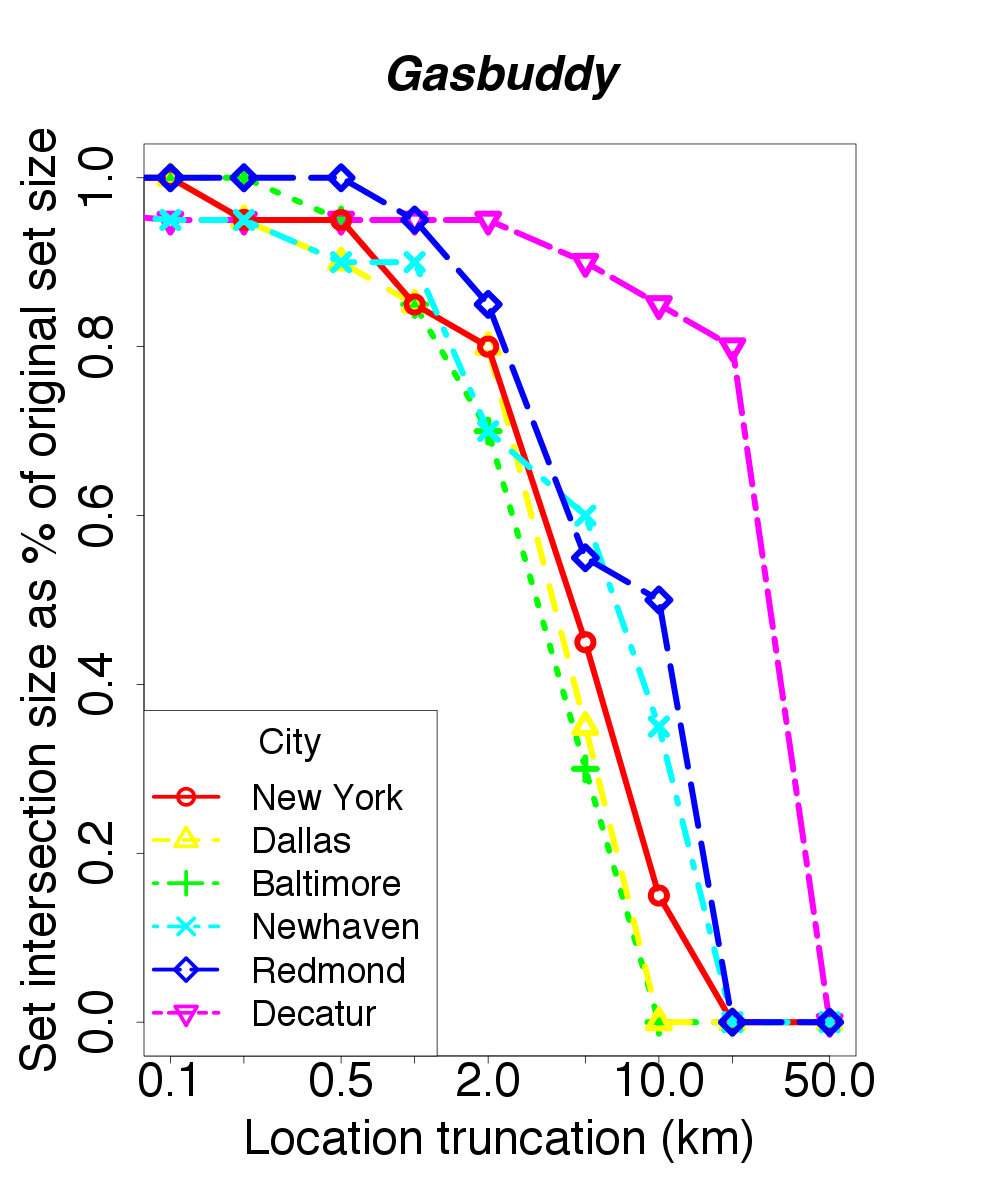
\includegraphics[width=\textwidth]
                      {data/gasbuddy/plots/medians_across_city_si_20}
    \end{minipage}
    
    % [width=.6\textwidth]
    \begin{minipage}{2in}
      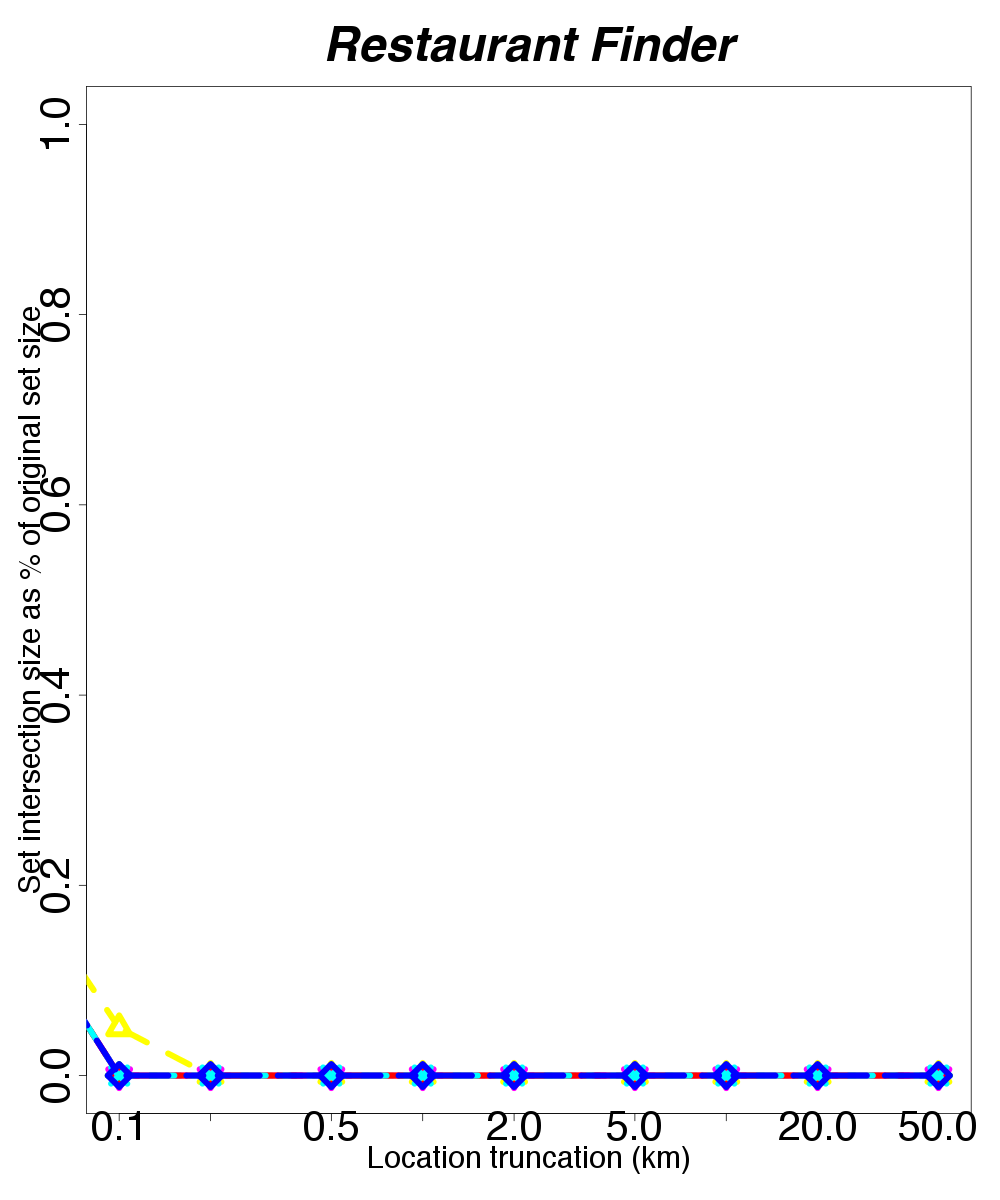
\includegraphics[width=\textwidth]
                      {data/restaurant_finder/plots/medians_across_city_si_20}
    \end{minipage}
    
    \begin{minipage}{2in}
      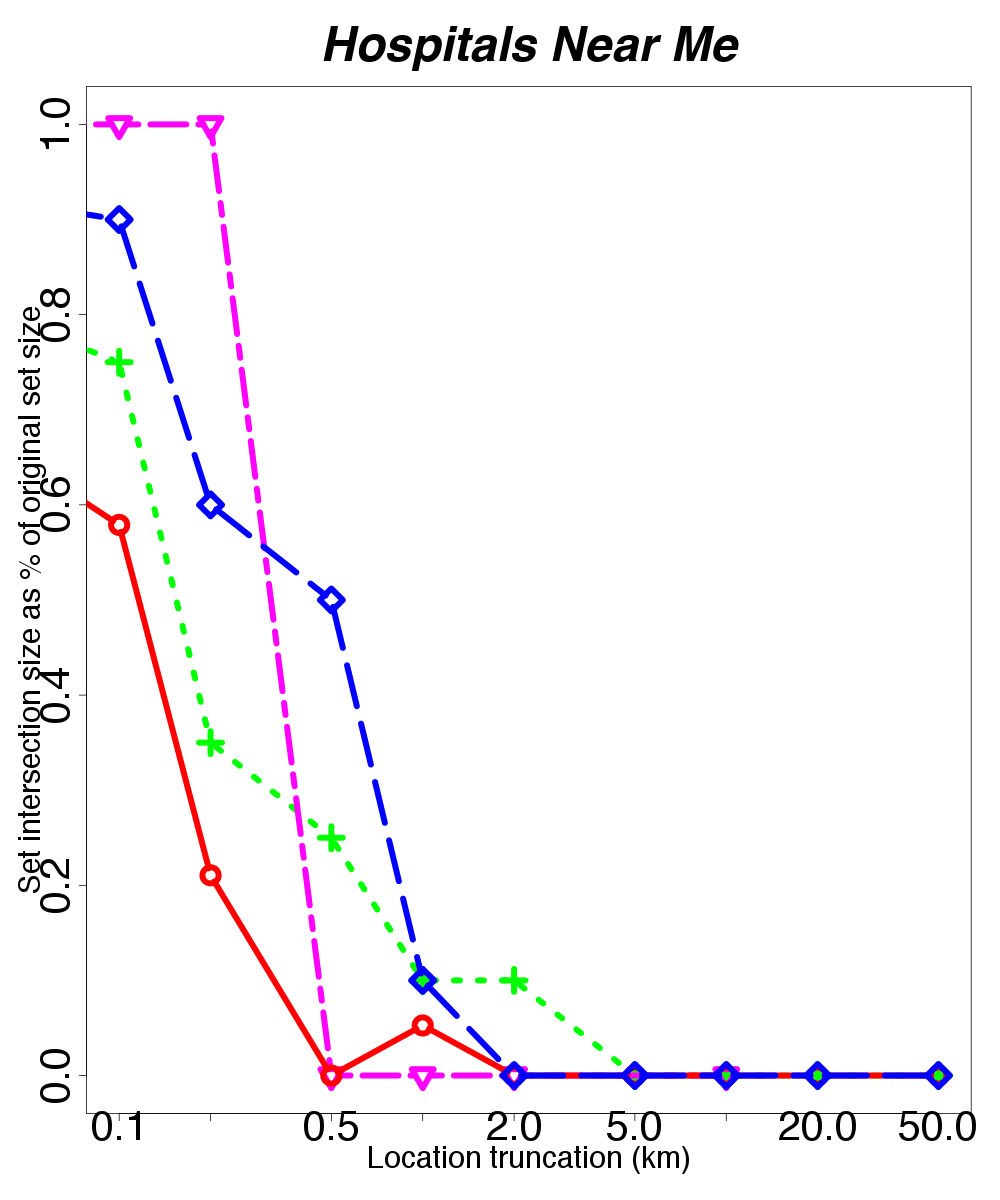
\includegraphics[width=\textwidth]
                      {data/hospitals/plots/medians_across_city_si_20}
    \end{minipage}
    
    \\
    \begin{minipage}{2in}
      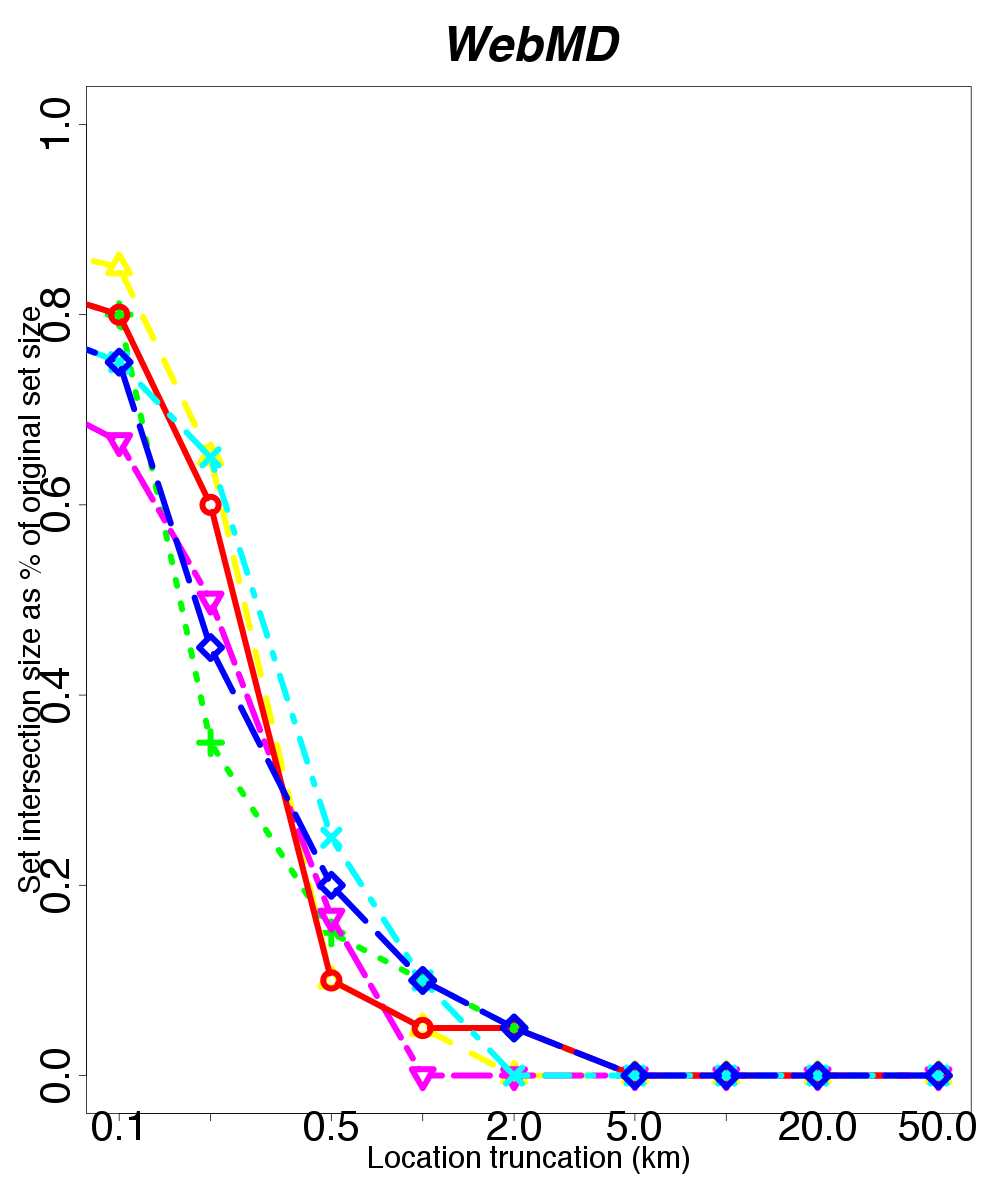
\includegraphics[width=\textwidth]
                      {data/webmd/plots/medians_across_city_si_20}
    \end{minipage}
    
    \begin{minipage}{2in}
      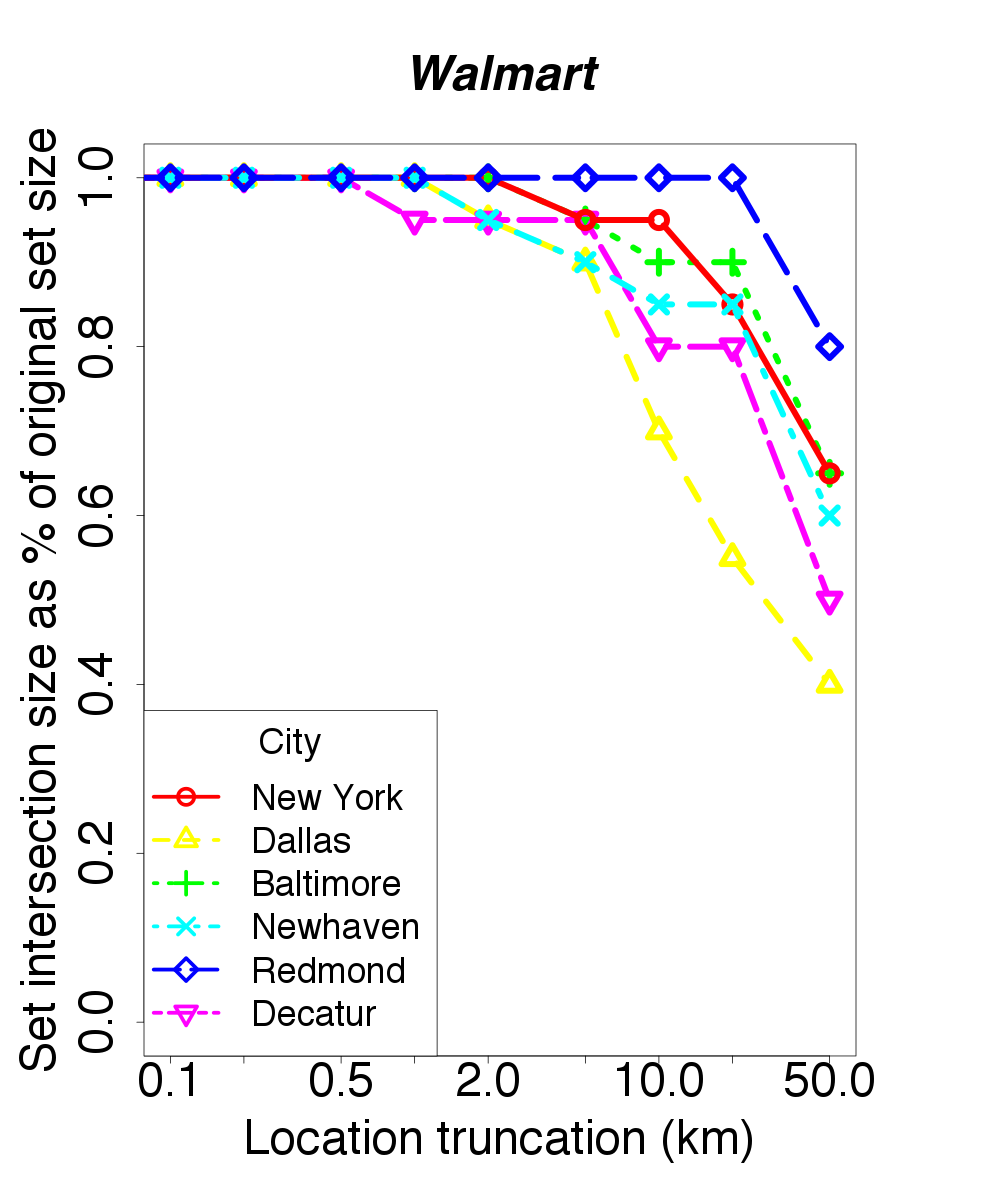
\includegraphics[width=\textwidth]
                      {data/walmart/plots/medians_across_city_si_20}
    \end{minipage}
    
    \begin{minipage}{2in}
      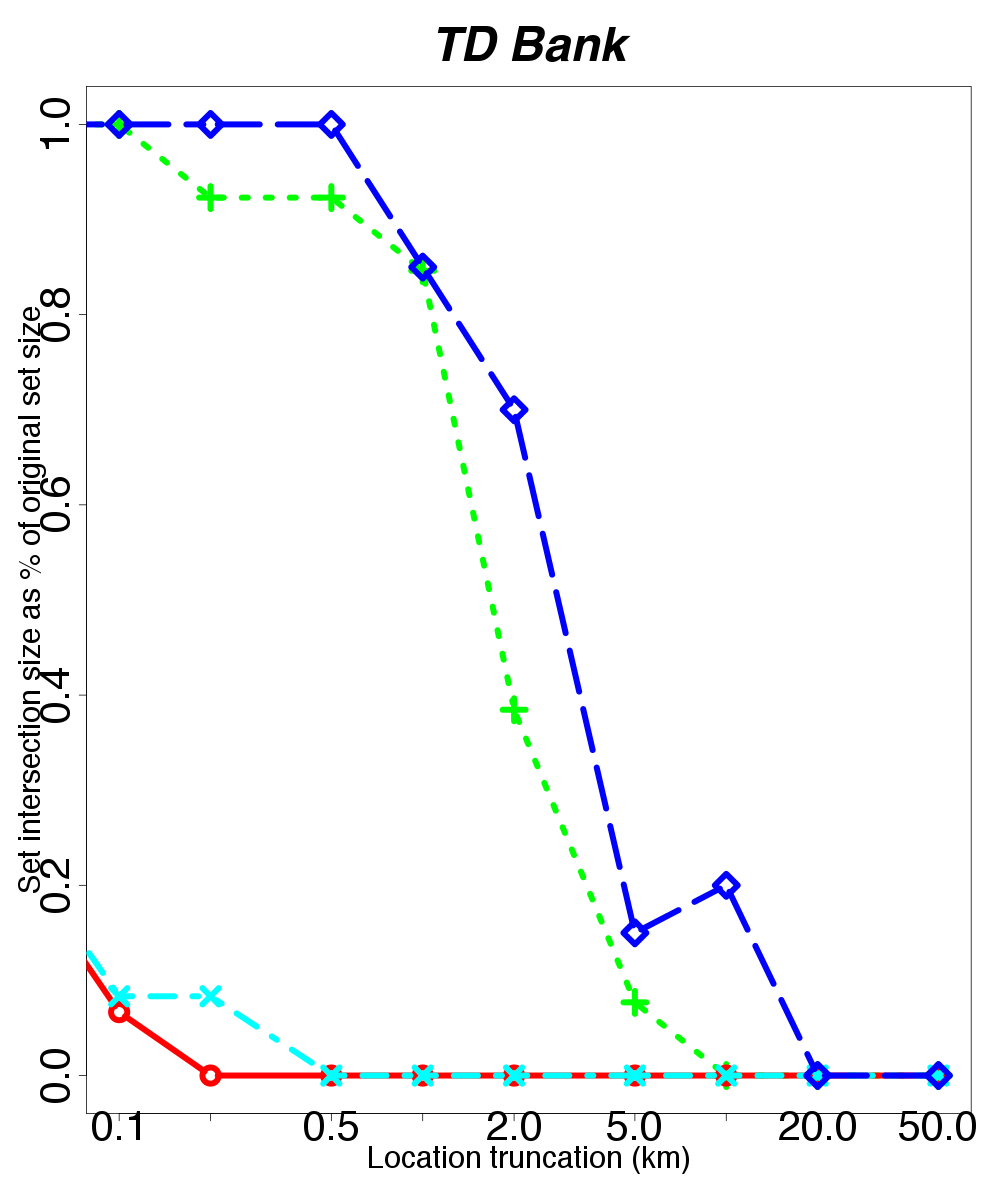
\includegraphics[width=\textwidth]
                      {data/tdbank/plots/medians_across_city_si_20}
    \end{minipage}
  \end{tabular}
  \caption{Graphs of median set intersection size versus
    truncation amount. Lower set intersection size indicates lower
    utility.}
  \label{fig:set-intersection-metric}
  \end{subfigure}

  \bigskip{}

  \begin{subfigure}{\textwidth}
 \small
 \centering
 \begin{tabular}{|l||r|r|r|r|r|r|}
 \hline
 & New York & Dallas & Baltimore & New Haven & Redmond & Decatur \\
 \hline
 \hline
 Gasbuddy & 5 & 5 & 2 & 2 & 5 & 50 \\
\hline
Restaurant Finder & 1 & 0.5 & 0.1 & 0.1 & 0.1 & 0.2 \\
\hline
Walmart & 50 & 10 & 50 & 50 & $\cdot$ & 50 \\
\hline
TD Bank & 10 & $\cdot$ & 50 & 20 & $\cdot$ & $\cdot$ \\
\hline
WebMD & 10 & 5 & 2 & 10 & 10 & 50 \\
\hline
Hospitals Near Me & 5 & $\cdot$ & 20 & $\cdot$ & 20 & $\cdot$ \\
\hline

\end{tabular}
 \caption{Largest truncation amount (km) before which the median set
   intersection size is lower than 80\%.}
 \label{fig:knee-points-set-cutoff}
  \end{subfigure}
  
  \caption{Set intersection size results.}
\end{figure*}


Figure~\ref{fig:add_distance} shows the results for the additional
distance metric applied to our subject apps.
Figure~\ref{fig:knee-points-additional-cutoff} shows, for each city
and each app, the last truncation amount before median additional
distance degrades beyond 1~km. More precisely, if $\Delta(s)$ is the
median additional distance under truncation $s$, then the chart lists
the $s_i$ such that $\Delta(s_i) \leq 1~km$ and $\Delta(s_{i+1}) >
1~km$ where $s_j$ is the sequence of location truncation amounts.

Note that the additional distance is undefined if a location
truncation produces a new closest location that was not present in the
original output list, as in this case we cannot compute how far the
new closest location is from the current location. In the charts,
undefined additional distances are omitted, as thus some lines end
before reaching the maximum truncation. This also limits the number of
points on which we can compute the cutoff.  For example, the Gasbuddy
app never causes the user to go more than 1 km out of the way in New York, 
so it is listed as $\cdot$ in Figure~\ref{fig:knee-points-additional-cutoff}.

From these plots, we can see that under the additional distance
metric, there is typically no change in app utility up to 1 or 2~km
truncation. Notice that this is
quite different behavior than under the edit distance metric,
where the edit distance is nonzero even with small amounts of 
location truncation.

%  This is because 
% our truncation will only happen in one direction:  (if you trace the 
% geographic position of the nominal input from the true input, it will 
% form a vector away from the true input): once a set of nearby locations 
% is passed, those locations will never possibly appear again as the top 
% output in the nominal list.
% \jeff{I don't understand the previous explanation, and the part of the
%   explanation I understand I don't believe. Can you explain this better?}

In most cases, the lack of change in additional distance is
meaningful, but in a few cases it only reveals the low density of
located objects. In particular, in Redmond, the TD Bank app can
sustain location truncation up to 50~km without any change, but
this occurs because the first result on the list is over 100 km~away. This
also happens in the Hospitals Near Me app, as there are relatively few
hospitals in any area.

Looking at Figure~\ref{fig:knee-points-additional-cutoff}, we see that
if a user is willing to go 1~km out of their way, then in most
locations apps can sustain truncation amounts of 5~km or
more. However, as with edit distance the effect is highly dependent on
density of objects, e.g., Gasbuddy and Restaurant Finder have 5~km
truncation as their limit (except in Decatur, which has fewer gas
stations), whereas other apps sometimes can be truncated to higher levels.

\subsection{Set Intersection}

Figure~\ref{fig:set-intersection-metric} shows the results for the set
intersection size metric, with the y-axis the percentage of the set
intersection size compared to the original set size.
Figure~\ref{fig:knee-points-set-cutoff} shows the truncation amount
after which the set intersection percentage drops below 80\% of the
original value. Analogously to above, this is the truncation amount
$s_i$ such that the percentage at $s_i$ is at least 80\%, and the
percentage at $s_{i+1}$ is less than 80\%.

Under this metric, we see similar behavior to the additional distance
metric. From the graphs, we see that Gasbuddy and Restaurant Finder
can sustain some truncation, but it drops off much faster than the
other apps. From the table, we see that much lower truncation amounts
can be sustained by Gasbuddy and Restaurant Finder before dropping
below a set intersection size of 80\%.
The table also shows that the Resaturant Finder app can be truncated 
more in New York than in other locations.  This is because the radius
we chose for New York (20 km) was greater than for other cities.  
Since restaurants are typically distributed densely around a city center,
we saw a lower density in New York than other cities.

% In the case of
% Restaurant Finder, we find that the data for New York can withstand
% more truncation than less populated cities.  This is because we choose
% a large radius for New York (in accordance with its size determined by
% a map).  For the other cities we choose smaller radii.  Since
% restaurants will be densely distributed in a city center, and we took
% a median of results, it makes sense that the data for the point in New
% York will withstand more truncation.

\subsection{Discussion}

Each of the three metrics applies in a different situations: edit
distance for when an exact order is desired, set intersection for when
a user wants to find any number of locations close by, and additional
distance for when a user wants to find a nearest location to visit.
The general trends for all three are similar: the metrics are much
more forgiving in less dense areas, which makes intuitive sense. In
terms of absolute values of truncation that can be sustained, we see
that edit distance is the least permissive, as very small changes have
large effects. (We did not include a table like
Figure~\ref{fig:knee-points-additional-cutoff}
or~\ref{fig:knee-points-set-cutoff} for edit distance because we have
no intuition of what a reasonable cutoff would be.) The next most
restrictive metric is set intersection size, and the most permissive
metric is additional distance.

\section{Related Work}

There is a large body of work that focuses on increasing location
privacy, though we are aware of no other work that directly measures
utility of mobile Android apps.

The Cach\'{e} system \cite{Amini:2010} caches and prefetches
content from a server, obfuscating the user's location at the cost of
potentially stale content and higher bandwidth.  Additionally,
application writers must specify rules for caching up front.  The
system caches data for a set of regions, quantizing the user's location 
as in our approach.  
The authors note that app utility will be impacted by their technique, 
but they do not measure it explicitly.

Shokri et al. \cite{Shokri:2011} present a systematic approach to
quantifying Location Privacy Preserving Mechanisms (LPPMs).  They also
present a tool (in the form of an updating meter on the user's device)
to continuously inform a user of their privacy.  In our work, we implemented a simple
truncation-based LPPM (corresponding to a technique they call
\emph{precision reduction}), and use this to study
utility as a function of the degree of truncation. As future work, we
may consider evaluating the utility of other policies from their
system.

In follow up work, Shokri et al. \cite{Shokri:2012} present an
optimal strategy to prevent localization attacks, based on bounding
the probability that an attacker can learn the
precise location of a user at a given time.  
Their analysis formulates location privacy as a Bayesian Stackelberg 
game, where a user chooses a location cloaking strategy without 
knowing which potential adversary they will face.
While their analysis considers service quality, they use metrics that do 
not clearly map to utility, such as euclidean distance from the 
true location (rather than the actual effect of the change on the service).

Our study focuses on privacy for a single user at a stationary point.
Allowing the app to collect traces of data reveals much more
information \cite{Gruteser:2005}, \cite{Golle:2009}.  Much of the
existing work \cite{Beresford:2004}, \cite{Bettini:2005},
\cite{Hoh:2005}, \cite{Gruteser:2003} focuses on $k$-anonymity: if a
user is making a query to a location based service, they can only be
identified to be within a set of $k$ potential users.  
One popular
technique is to use mix zones \cite{Beresford:2004}: once a user enters 
a designated area their location information becomes ``mixed'' with 
others in that same area.  This technique requires a trusted middleware 
layer (to properly mix location data) and requires these mix zones 
to be defined.  In contrast, location truncation can be done locally
on a mobile device.

None of these previous approaches study the impact of location privacy
on app utility.  The work that comes closest is by Shokri et
al. \cite{Shokri:2012}, but while that framework considers utility as
an element of their models, it is not directly measured on apps.  Our
work is complementary: we focus not on optimal obfuscation techniques,
but rather we fix an obfuscation strategy and study how utility
changes under that technique.  As future work, we intend to couple our 
empirical utility functions with the theoretical models presented by
Shokri et al.
Doing so would allow us to determine bounds for $k$ and allow us study 
how the optimal strategies presented by Shokri et al.
are affected.

%% \jeff{
%% Many free apps include ads, but at the occasional
%% expense of end users \cite{wei:pmp2012}.  The work by
%% \cite{json:spsm12} proposes how to rewrite apps to remove ad libraries.
%% }

\section{Conclusion}

We presented an empirical study of how location truncation affects
mobile app utility. We began by examining how Android apps use
location. Across the apps we looked at, we found that the second most
common pattern is using the current location to list various sorts of
nearby objects. The most common pattern, location-targeted ads, is not
amenable to evaluating utility. We then used Dr.~Android and Mr.~Hide,
a previously developed system, to implement \fuzzer{}, a tool that
modifies existing apps' bytecode to use truncated location
information. We designed an experiment in which we measured the effect
of a range of location truncations (from 0~km to 50~km) on 60
points randomly chosen from various locales (from population 6,000
Decatur, TX to population 8.2 million New York, NY). We identified three
metrics that approximate app utility: edit distance, set intersection
size, and additional distance. We found that, under these metrics, the
factor that most determines the utility--truncation amount tradeoff is
the density of objects being returned by the app, and that in many
cases, location can be truncated significantly without losing much
utility. To our knowledge, our work provides the first end-to-end
evaluation of how location truncation affects Android app utility.

\bibliographystyle{IEEEtran}
\bibliography{paper}

\end{document}
